\documentclass[12pt]{article}
\RequirePackage{amsthm,amsmath,amsbsy,amsfonts}
\usepackage{graphicx}
%\usepackage{enumerate}
\usepackage{natbib}
\usepackage{url} % not crucial - just used below for the URL 
\usepackage{placeins}

%\pdfminorversion=4
% NOTE: To produce blinded version, replace "0" with "1" below.
\newcommand{\blind}{0}

% DON'T change margins - should be 1 inch all around.
\addtolength{\oddsidemargin}{-.5in}%
\addtolength{\evensidemargin}{-.5in}%
\addtolength{\textwidth}{1in}%
\addtolength{\textheight}{1.3in}%
\addtolength{\topmargin}{-.8in}%


\begin{document}
	
	%\bibliographystyle{natbib}
	
	\def\spacingset#1{\renewcommand{\baselinestretch}%
		{#1}\small\normalsize} \spacingset{1}
	
	
	%%%%%%%%%%%%%%%%%%%%%%%%%%%%%%%%%%%%%%%%%%%%%%%%%%%%%%%%%%%%%%%%%%%%%%%%%%%%%%
	
	\if0\blind
	{
		\title{\bf Drift Removal for Time Series Data Using Quantile Trend Filtering}
		\author{Halley Brantley\thanks{
				Department of Statistics, North Carolina State University, Raleigh, NC 27695 (E-mail: hlbrantl@ncsu.edu)} \,
			Joseph Guinness\thanks{
				Department of Biological Statistics and Computational Biology, Cornell University, Ithaca, NY 14853 (E-mail: guinness@cornell.edu )} \,
			and
			%    and
			Eric C. Chi\thanks{Department of Statistics, North Carolina State University, Raleigh, NC 27695 (E-mail: eric$\_$chi@ncsu.edu).}    \\}
		\date{}
		\maketitle
	} \fi
		
	\if1\blind
	{
		\bigskip
		\bigskip
		\bigskip
		\begin{center}
			{\LARGE\bf Title}
		\end{center}
		\medskip
	} \fi
	
	\bigskip
	\begin{abstract}
		The text of your abstract.  200 or fewer words.
	\end{abstract}
	
	\noindent%
	{\it Keywords:}  3 to 6 keywords, that do not appear in the title
	\vfill
	
	\newpage
	\spacingset{1.5} % DON'T change the spacing!
	\section{Introduction}
	\label{sec:intro}
	
	We are interested in the problem posed by \cite{thoma2016south} concerning low-cost air pollutant sensors. Researchers at the U.S. Environmental Protection Agency have built prototypes of low-cost sensors that provide an un-calibrated measure of volatile organic compounds (VOCs) and hazardous air pollutants (HAPs) at a 1 second time resolution. To reduce cost and power consumption, the temperature and relative humidity of the air presented to the photoionization detectors (PIDs) is not controlled. A result the output signal exhibits a slowly varying baseline drift (minutes to hours). The purpose of these sensors is to protect the fenceline of industrial facilities by detecting whether VOC emissions from a local source are present and providing wind and concentration data to help identify the source and speed repairs.   
	
	There have been a number of occasions when researchers have sought to estimate the trend in the quantiles of a random variable over time or another co-variate given noisy observations of that variable. \cite{nychka1995nonparametric} estimated smooth quantile curves of friction profiles of syringes in order to automate their quality assessment procedures. \cite{Ning2014} proposed a method for separating chromatogram peaks from the smooth baseline and noise present in the measurements. \cite{brantley2014mobile} examined air pollutant measurements collected using a monitoring vehicle and proposed using a smooth baseline trend as an estimate of regional background pollution.    	
	
	A variety of approaches have been proposed for estimating quantile trends. \cite{Koenker1978} was the first to propose the use of the check loss function to estimate conditional quantiles. Given a design matrix $\mathbf{X} \in \mathbb{R}^{n \times p}$ and continuous responses $y \in \mathbb{R}^n$, we estimate a regression vector $\theta \in \mathbb{R}^p$ so that $\mathbf{X}\theta$ is a good approximation of the $\tau$th quantile of $y$ conditional on $x$. The regression vector $\theta$ is estimated by finding the minimizer of $\rho_{\tau}(y-X\theta)$ where $\rho_{\tau}(y) = \sum_{i=1}^n y_i(1-\mathbf{I}(y_i<0))$ is the check-loss function and $\mathbf{I}$ is the indicator function.  
	
	In the trend filtering problem \citep{Kim2009, Tib2014}, one is interested in finding an adaptive polynomial approximation to noisy data $y \in \mathbb{R}^n$ by solving the following convex problem.
	\begin{eqnarray}
	\underset{\theta}{\arg\min}\; \frac{1}{2n} \lVert y - \theta \rVert_2^2 + \lambda \lVert \mathbf{D}^{(k+1)}\theta \rVert_1,
	\end{eqnarray}
	where $\lambda \geq 0$ is a regularization parameter that trades off the emphasis on the data fidelity term and the matrix $\mathbf{D}^{(k+1)} \in \mathbb{R}^{(n - k -1) \times n}$ is the discrete difference operator of order $k+1$. To understand the purpose of penalizing $\mathbf{D}^{(k+1)}$ consider the difference operator when $k = 0$.
	\begin{eqnarray}
	\mathbf{D}^{(1)} = \begin{pmatrix}
	-1 & 1 & 0 & \cdots & 0 & 0 \\
	0 & -1 & 1 & \cdots & 0 & 0 \\
	\vdots & & & & & \\
	0 & 0 & 0 & \cdots & -1 & 1 \\
	\end{pmatrix}
	\end{eqnarray}
	Thus, $\lVert \mathbf{D}^{(1)}\theta \rVert_1 = \sum_{i=1}^{n-1} \lvert \theta_i - \theta_{i+1} \rvert$ which is just total variation denoising in one dimension. The penalty incentivizes solutions which are piece-wise constant. For $k \geq 1$, the difference operator $\mathbf{D}^{(k+1)} \in \mathbb{R}^{(n-k-1) \times n}$ is defined recursively as follows
	\begin{eqnarray}
	\mathbf{D}^{(k+1)} & = & \mathbf{D}^{(1)}\mathbf{D}^{(k)}.
	\end{eqnarray}
	By penalizing the $k+1$ fold composition of the discrete difference operator, we obtain solutions which are piecewise polynomials of order $k$.
	
	We propose to use the trend filtering penalty with the check loss function to produce a non-parametric quantile regression estimate for removing trends in time series. The formulation was proposed by \cite{Kim2009} as a possible extension of $\ell_1$-trend filtering but not studied. Moreover we extend the basic framework to ensure non-crossing while modeling multiple quantiles. We also implement a parallel ADMM algorithm for series that are too large to be computed simultaneously and proposed a modified criteria for choosing the smoothing parameter. We demonstrate through simulation studies that our proposed model provides better or comparable estimates of non-parametric quantile trends than existing methods and is a more effective method of drift removal for low-cost air quality sensors. 
	

	\section{Methods}
	
	\subsection{Quantile Trend Filtering}
	
	We combine the ideas of quantile regression and trend filtering, namely consider the case where the design $\mathbf{X}$ is the identity matrix. For a single quantile level $\tau$ the estimation of the quantile trend filtering model can be posed as the following optimization problem.
	\begin{eqnarray}
	\label{eq:quantile_trend}
	\underset{\theta}{\min}\; \frac{1}{n} \sum_{i=1}^n \rho_\tau(y_i - \theta_i) + \lambda \lVert \mathbf{D}^{(k)} \theta \rVert_1,
	\end{eqnarray}
	where $\lambda$ is a non-negative tuning parameter. As with the classic quantile regression, the quantile trend filtering problem is a linear program which can be solved by a number of free or commercial solvers. In many cases, including ours, we are interested in estimating multiple quantiles simultaneously. We also want to ensure that our quantile estimates are valid by enforcing the constraint that if $\tau_2 > \tau_1$ then $Q(\tau_2) \ge Q(\tau_1)$. Given quantiles $\{\tau_1, ..., \tau_J\}$ such that $\tau_1 < \tau_2 < ... < \tau_J$, the optimization problem becomes 
	
	\begin{eqnarray}
	\label{eq:quantile_trend}
	\underset{\theta}{\min}\; \sum_{j=1}^J \left [\frac{1}{n} \sum_{i=1}^n \rho_{\tau_j}(y_i - \theta_{ji}) + 
	\lambda_j \lVert \mathbf{D}^{(k)} \theta_j \rVert_1 \right ] \\
	 \text{subject to: }\; \theta_{1i} \le \theta_{2i} \le ... \le \theta_{Ji} \text{ for all } i,
	\end{eqnarray}
	
	where $\theta = (\theta_1, ..., \theta_J)$ and $\theta_j \in \mathcal{R}^n$. The additional constraints are linear in the parameters so the non-crossing quantile trends can still be estimated by a number of available solvers. 
	
	The number of parameters to be estimates is equal to the number of observations multiplied by the number of quantiles of interest. As the size of the data and the number of quantiles grows, all solvers will eventually break. 
	
	\subsection{ADMM for Big Data}
	
	To our knowledge, no one has addressed the problem of finding smooth quantile trends of series that are too large to be processed simultaneously. We propose an alternating direction method of multipliers (ADMM) algorithm for solving large problems in a piecewise fashion. The ADMM algorithm is fully described by \cite{boyd2011distributed, gabay1975dual, glowinski1975approximation}. We apply the consensus ADMM algorithm to the the quantile regression trend filtering problem, 
	\begin{equation}
	\text{minimize } \rho_\tau(y-\theta) + \lambda||D^{(k)}\theta||_1\\
	\end{equation}
	where $y,\theta \in \mathbf{R}^n$, $y$ is the observed data, $\rho_{\tau}(u) = \sum_i(\tau - I(u_i < 0))u_i$ is the check loss function corresponding to quantile level $\tau$ and $D^{(k)}$ is the discrete differencing matrix of order $k$ and $\lambda$ is a tuning parameter that controls smoothness. We first re-parameterize $\phi = y-\theta$ so the problem is
	\begin{equation}
	\text{minimize } \rho_\tau(\phi) + \lambda||D^{(k)}(y-\phi)||_1\\
	\end{equation}
	We further divide $\phi$ order to solve smaller problems: Defining
	\begin{align}
	&\phi_1 = (\phi_{11}, \phi_{12})\\
	&\phi_2 = (\phi_{21}, \phi_{22}, \phi_{23})\\
	&\phi_3 = (\phi_{31}, \phi_{32})\\
	&\phi = (\phi_{11}, \phi_{12}=\phi_{21}, \phi_{22}, \phi_{23}=\phi_{31}, \phi_{32}) \\
	\end{align}
	Dividing $y$ similarly, the problem then becomes 
	\begin{align}
	&\text{minimize } \sum_{i=1}^3 \rho_\tau(\phi_i) + \lambda||D^{(k)}(y_i-\phi_i)||_1\\
	&\text{subject to: } \phi_{12}=\phi_{21}, ~~ \phi_{23}=\phi_{31}\\
	\end{align}
	We can further simplify by defining 
	\begin{align}
	&\overline{\phi} = (\phi_{11}, \frac{\phi_{12}+\phi_{21}}{2}, \phi_{22}, \frac{\phi_{23}+\phi_{31}}{2}, \phi_{32}) \\
	&\overline{\phi_1} = (\phi_{11}, \frac{\phi_{12}+\phi_{21}}{2})\\
	&\overline{\phi_2} = ( \frac{\phi_{12}+\phi_{21}}{2}, \phi_{22}, \frac{\phi_{23}+\phi_{31}}{2})\\
	&\overline{\phi_3} = (\frac{\phi_{23}+\phi_{31}}{2}, \phi_{32})
	\end{align}
	so the problem becomes
	\begin{align}
	&\text{minimize } \sum_{i=1}^3 \rho_\tau(\phi_i) + \lambda||D^{(k)}(y_i-\phi_i)||_1\\
	&\text{subject to: } \phi_{i}=\overline{\phi_i}\\
	\end{align}
	The augmented Lagrangian for this problem is 
	\begin{align}
	&L_\gamma(\phi_1,\phi_2, \phi_3, \overline{\phi_1}, \overline{\phi_2}, \overline{\phi_3}, \omega) = \\
	&\sum_{i=1}^3 \rho_\tau(\phi_i) + \lambda||D^{(k)}(y_i-\phi_i)||_1 + \omega_i^T(\phi_i - \overline{\phi_i}) + \frac{\gamma}{2}||\phi_i - \overline{\phi_i}||_2^2
	\end{align}
	The ADMM updates are then given by
	\begin{align}
	&\phi_i^{k+1} = \arg\min_{\phi_i}\rho_\tau(\phi_i) + \lambda||D^{(k)}(y_i-\phi_i)||_1 + \omega_i^{kT}(\phi_i - \overline{\phi_i}^k) + \frac{\gamma}{2}||\phi_i - \overline{\phi_i}^k||_2^2\\
	&\omega_i^{k+1} = \omega_i^{k} + \gamma(\phi_i^{k+1} - \overline{\phi_i}^{k+1})
	\end{align}
	The $\phi_i$ updates can be obtained using a quadratic program solver such as Gurobi and can be obtained in parallel. 
	
	\pagebreak 
	
	\begin{figure}[!h] 
		\caption{Windows fit separately compared to simultaneous fit, no signal present.}
		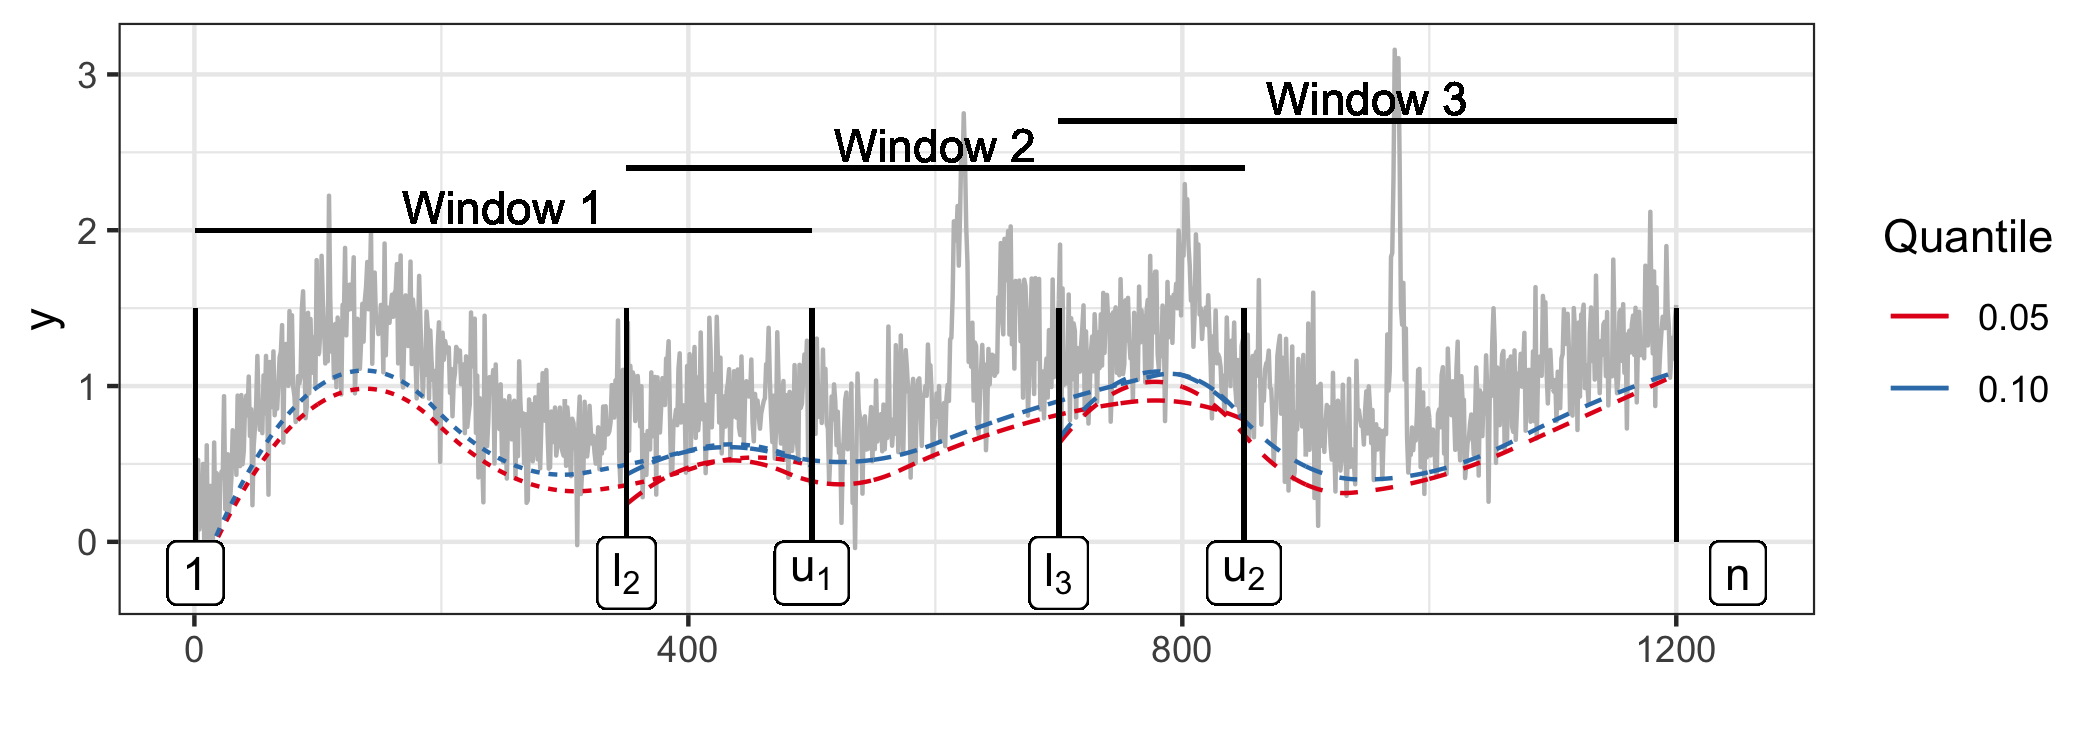
\includegraphics[width = \linewidth]{Figures/overlapping_windows.png}
	\end{figure}
	
	\begin{figure}[!h] 
		\caption{Windows fit with 150 iterations of ADMM, no signal present.}
		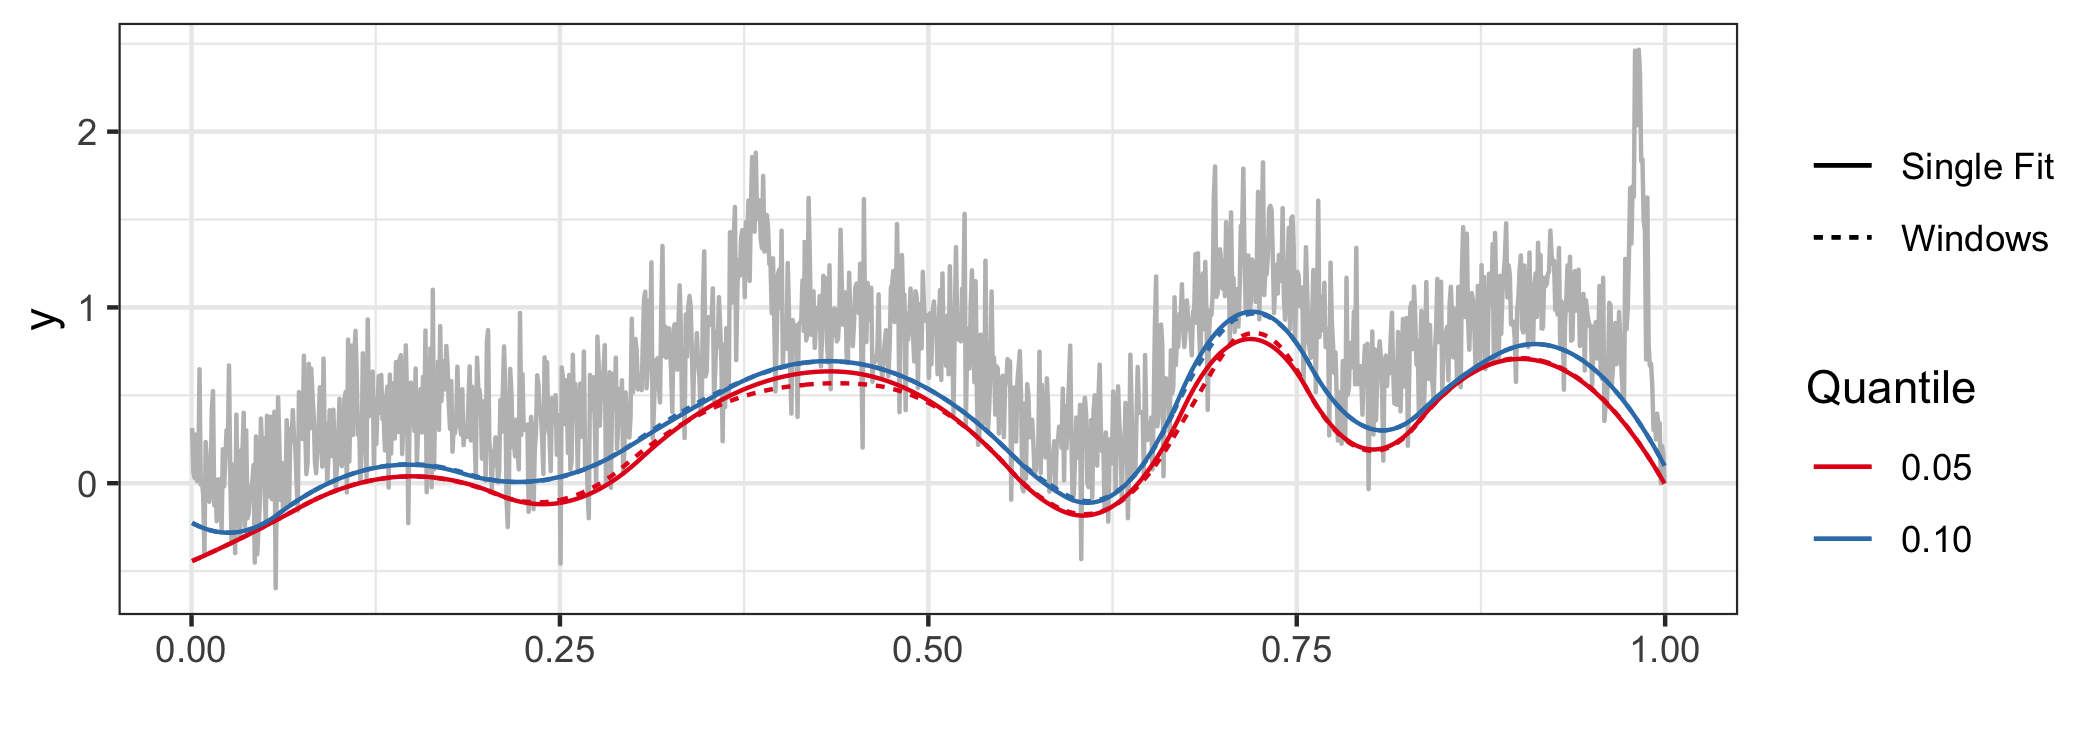
\includegraphics[width = \linewidth]{Figures/admm_windows.png}
	\end{figure}
	

	We conducted timing experiments to show the advantages of using our ADMM algorithm on large datasets. We use 2 windows for each data size with an overlap of 2000 and two iterations of the algorithm after the initial estimates. 
	
	\begin{figure}[!h] 
		\caption{Timing experiments comparing quantile trend filtering on a single window versus 2 windows by data size.}
		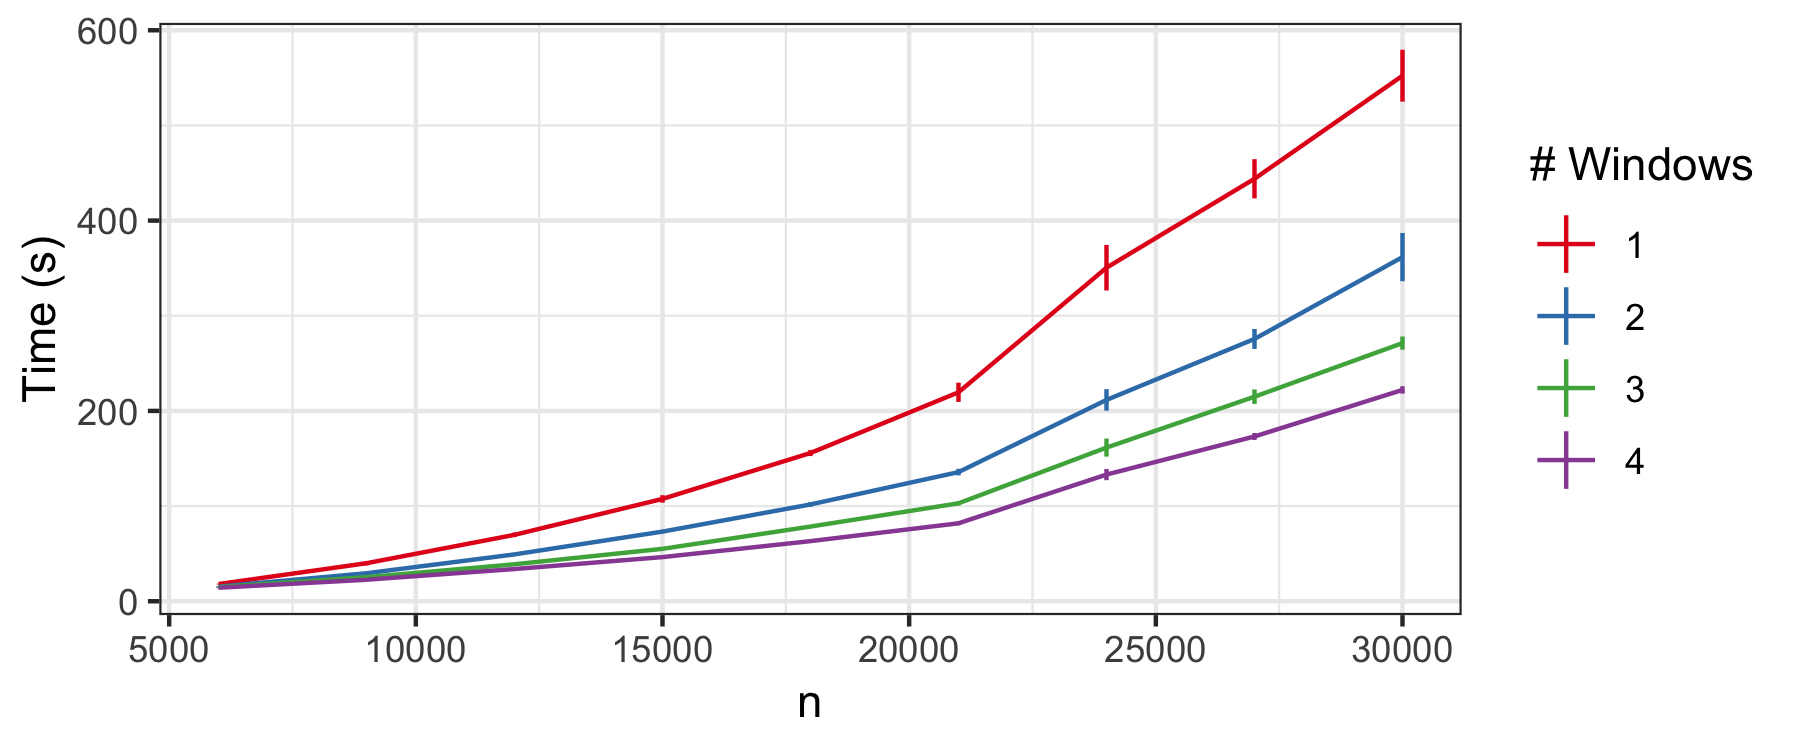
\includegraphics[width = \linewidth]{Figures/Fig_timing_experiment.png}
	\end{figure}

	\subsection{Smoothing parameter choice}
	Our method can easily handle missing data by changing the check loss function to output 0 for missing values. This allows us to leave out validation observations that can be used to select the tuning parameter $\lambda$ and to compare method performance on real data. A number of methods have been proposed for selecting the quantile regression smoothing spline tuning parameter \cite{yuan2006gacv}.  \cite{KoenkerNgPortnoy1994} relate $\lambda$ to the number of interpolated points $p_{\lambda} = \sum I(y_i = \widehat{g}_i(x_i))$, which can be thought of as active knots, they propose the Schwarz criterion for the selection of $\lambda$
	\begin{equation}
	\mbox{SIC}(p_{\lambda}) = \log[n^{-1}\sum\rho_{\tau}(y_i - \widehat{g}(x_i))] + \frac{1}{2n}p_{\lambda}\log n
	\end{equation}
	
	The traditional Bayesian Information Criterion (BIC) is given by 
	\begin{equation}
	\mbox{BIC}(s) = -2\log(L\{\hat{\theta}(s)\}) + \nu(s)\log n 
	\end{equation}	
	where $\theta(s)$ is the parameter $\theta$ with those components outside $s$ being set to 0, and $\nu(s)$ is the number of components in $s$. If we assume an asymmetric Laplace likelihood $L(y|\theta) = \left(\frac{\tau^n(1-\tau)}{\sigma}\right)^n\exp\left\{-\sum_i\rho_\tau(\frac{y_i - \theta_i}{\sigma})\right\}$ and the number of non-zero elements of $D\theta$ as $df$
	\begin{equation}
	\mbox{BIC}(df) = 2\sum_i\frac{1}{\sigma}\rho_{\tau}(y_i-\theta_i) + \mbox{df}\log n
	\end{equation} 
	We can choose any $\sigma>0$ and have found empirically that $\sigma =  \frac{1-|1-2\tau|}{2}$ produces stable estimates. \cite{chen2008} proposed the extended BIC for large parameter spaces 
	\begin{equation}
	\mbox{BIC}_{\gamma}(s) = -2\log(L\{\hat{\theta}(s)\}) + \nu(s)\log n  + 2\gamma\log{P\choose j,}~~\gamma \in [0,1]
	\end{equation}
	where $P$ is the total number of possible parameters and $j$ is the number of parameters included in given model. We used this criteria with $\gamma = 1$, $P=n-k$ where $k$ is the order of the differencing matrix and $j = \nu(s)$ is the number of non-zero entries in $D^{(k)}\theta$. 
	
	We used a single dataset to illustrate the difference between the scaled, unscaled and extended BIC criteria. 
	
	\begin{figure}[h!]
		\caption{Degrees of freedom (number of non-zero elements of $D\theta$) by $\log(\lambda)$.} 
		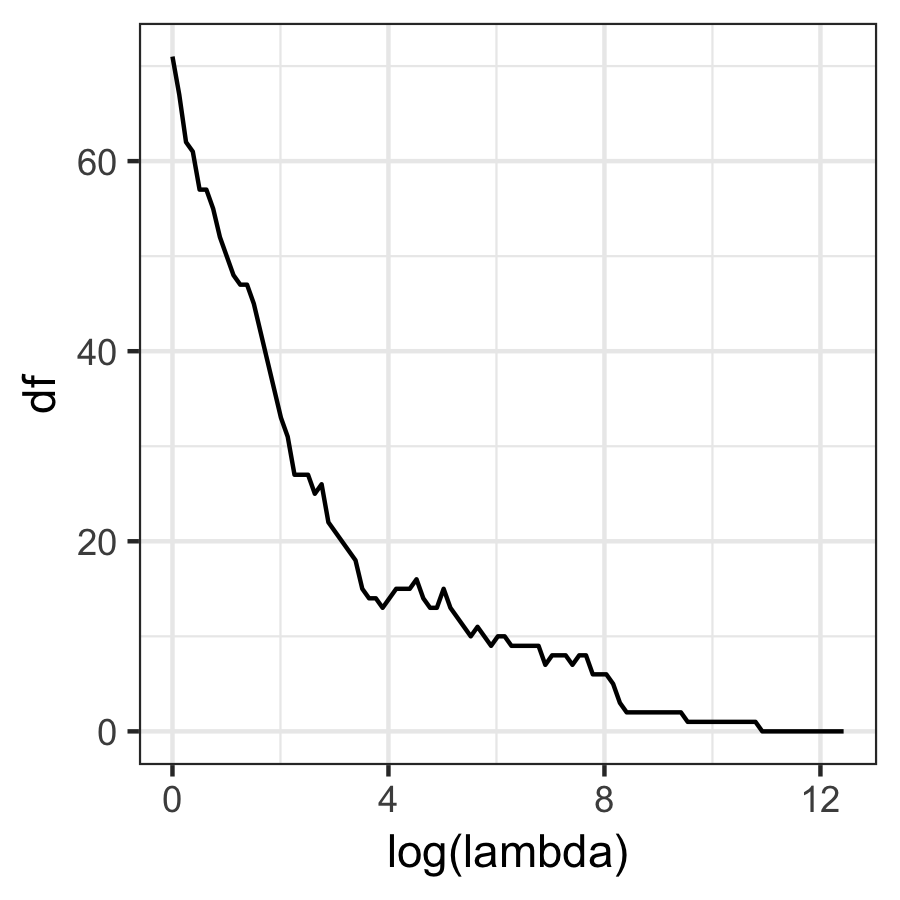
\includegraphics[width = 0.25\linewidth]{Figures/df_by_lambda.png}
		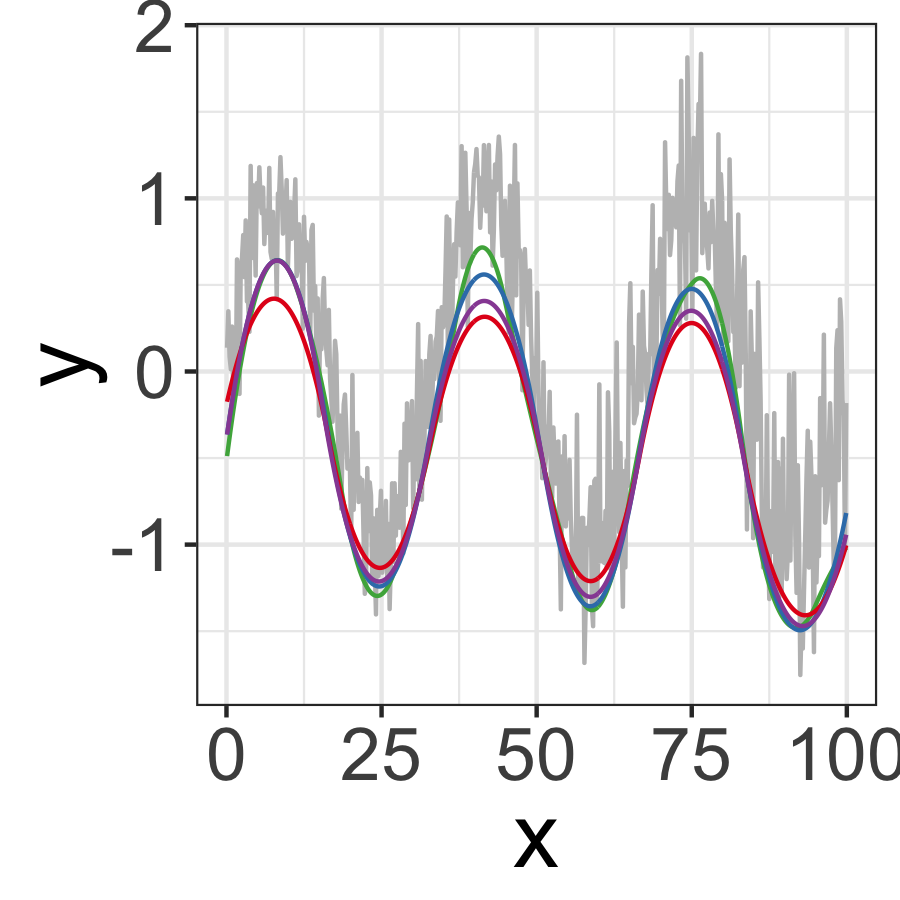
\includegraphics[width = 0.25\linewidth]{Figures/BIC_data.png}
		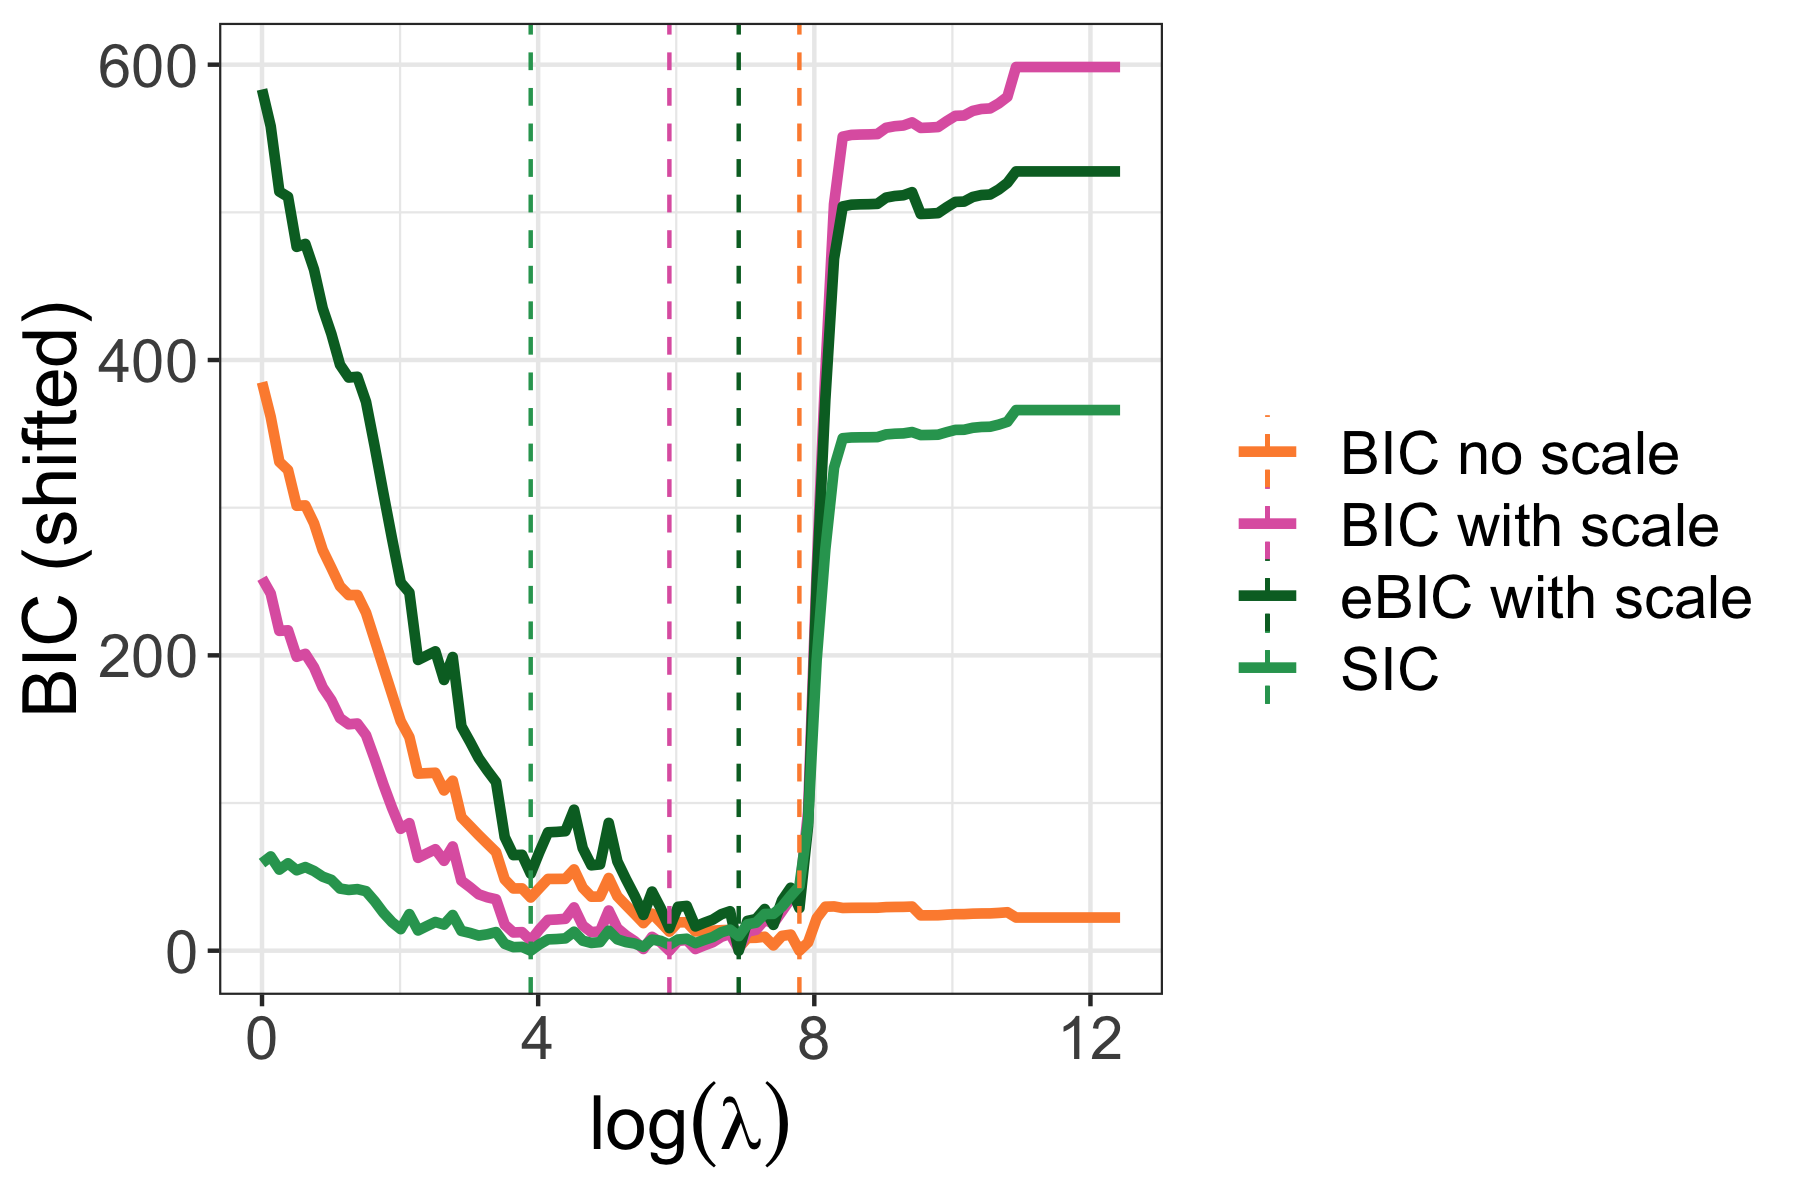
\includegraphics[width = 0.5\linewidth]{Figures/BIC_by_lambda.png}
	\end{figure}

	\section{Simulation Studies}
	
	\subsection{Estimating Quantiles}
	
	We compare the performance of our quantile trend filtering method with the three previously published methods using designs proposed by \cite{Racine2017}. The methods compared are: \texttt{npqw} which is the quantile-ll method described in \cite{Racine2017}, code was obtained from the author; \texttt{qsreg} in the \texttt{fields} R package and described in \cite{Oh2011}; \texttt{rqss} available in the \texttt{quantreg} package and described in \cite{KoenkerNgPortnoy1994}.  The smoothing parameter $\lambda$ for the \texttt{rqss} method is chosen using a grid search and minimizing the SIC criteria as described in \cite{KoenkerNgPortnoy1994}. We further compare three criteria for choosing the smoothing parameter for our detrend method: \texttt{detrendr\_SIC}: Our method where we minimize $\sum_i\rho_{\tau}(y_i - \theta_i) + \lambda||D\theta||_1$ and $\lambda$ is chosen using SIC \citep{KoenkerNgPortnoy1994}.  \texttt{detrendr\_valid}: Our method where lambda is chosen by leaving out every 5th observation as a validation data set and minimizing the evaluating the check loss function evaluated at the validation data. \texttt{detrendr\_eBIC}:  the new criteria we have proposed based on the extended BIC proposed by \cite{chen2008}. 
	 
	Three simulation designs from \cite{Racine2017} were considered. For all designs $X_i$ was generated as a uniformly spaced sequence in $[0,1]$ and the response $Y$ was generated as 
	$$Y_i = sin(2\pi x_i) + \epsilon_i(x_i)$$
	The three error distributions considered were 
	\begin{itemize}
		\item Gaussian: $\epsilon_i(x_i) \sim N\left(0, \left(\frac{1+x_i^2}{4}\right)^2\right)$
		\item Beta: $\epsilon_i \sim Beta(1, 11-10x_i)$
		\item Mixed normal: $\epsilon_i$ is simulated from a mixture of $N(-1,1)$ and  $N(1,1)$ with mixing probability $x_i$.
	\end{itemize}
	\begin{figure}
		\caption{Simulated data with true quantiles $\tau \in \{0.01, 0.05, 0.25, 0.5, .75, 0.95, 0.99\}$}	
		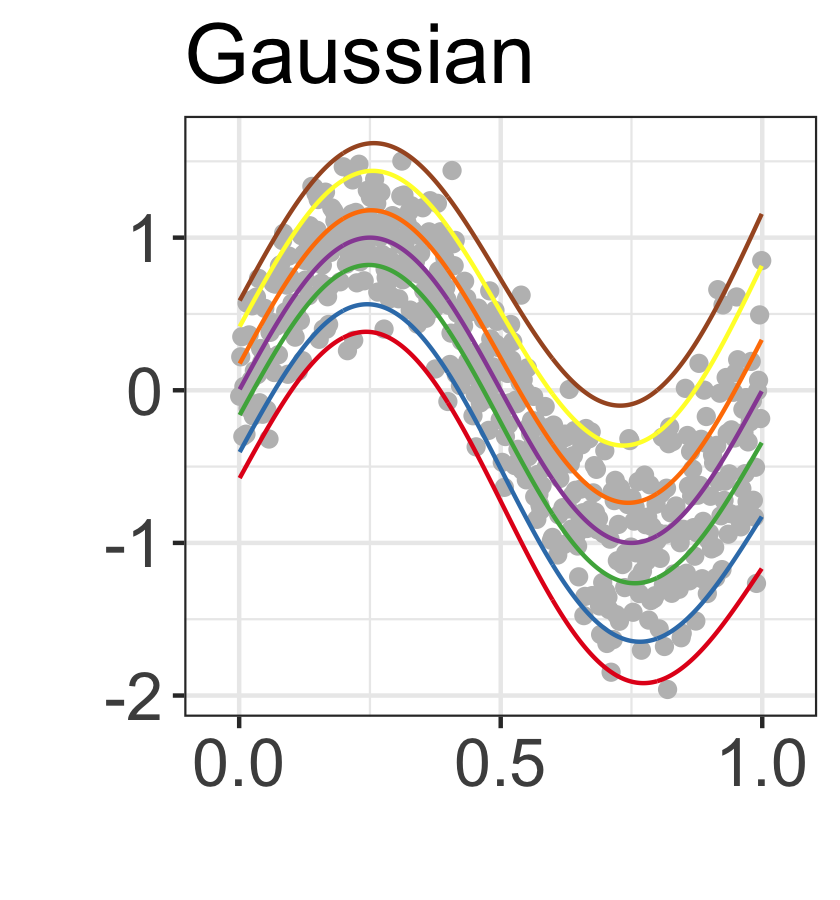
\includegraphics[width=.28\linewidth]{Figures/gaus.png}
		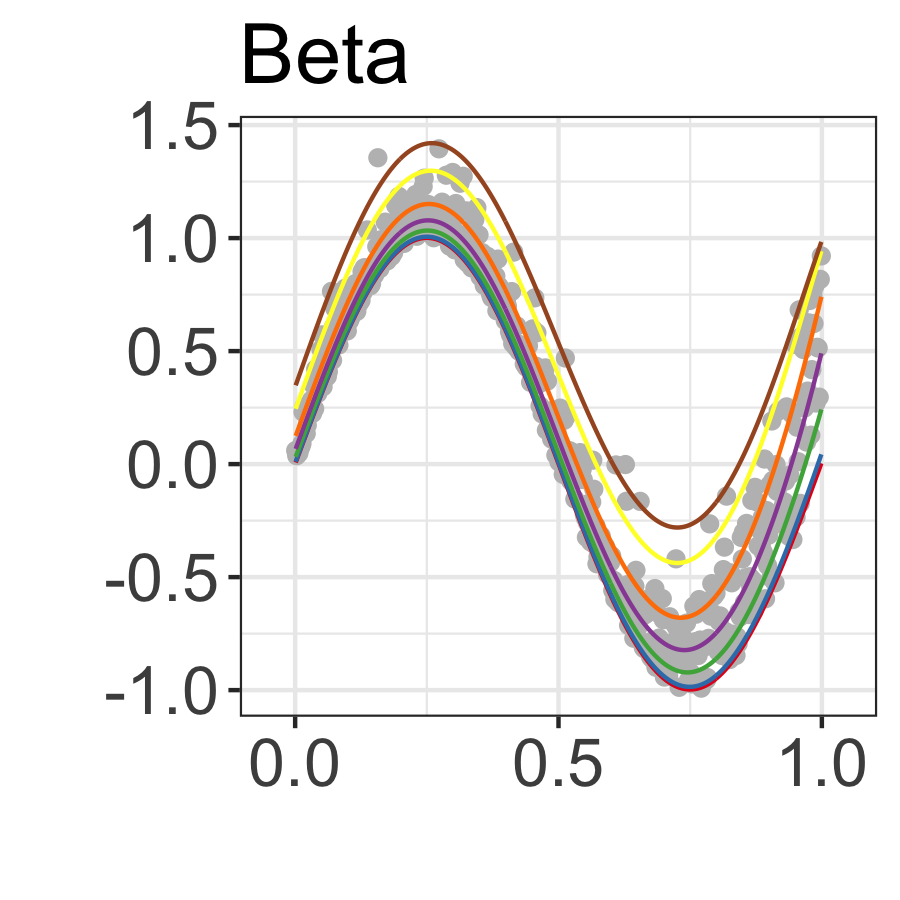
\includegraphics[width=.3\linewidth]{Figures/shapebeta.png}
		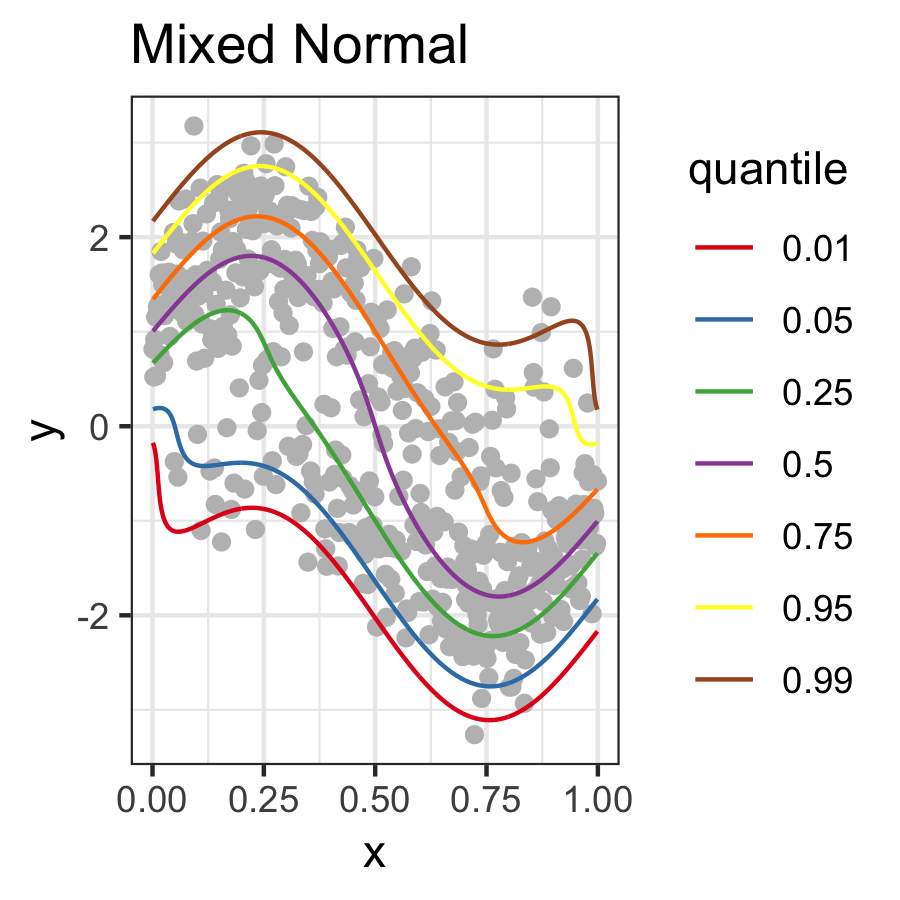
\includegraphics[width=.45\linewidth]{Figures/mixednorm.png}
	\end{figure}
	
	100 datasets were generated of sizes 300, 500 and 1000. The MSE was calculated as $\frac{1}{n}\sum_i (\hat{q}_{\tau}(x_i) - q_\tau(x_i))^2$. The plots below show the mean MSE $\pm$ twice the standard error by method, quantile level and sample size. 
	
	\begin{figure}
		\caption{RMSE by design, method, quantile and data size.}
		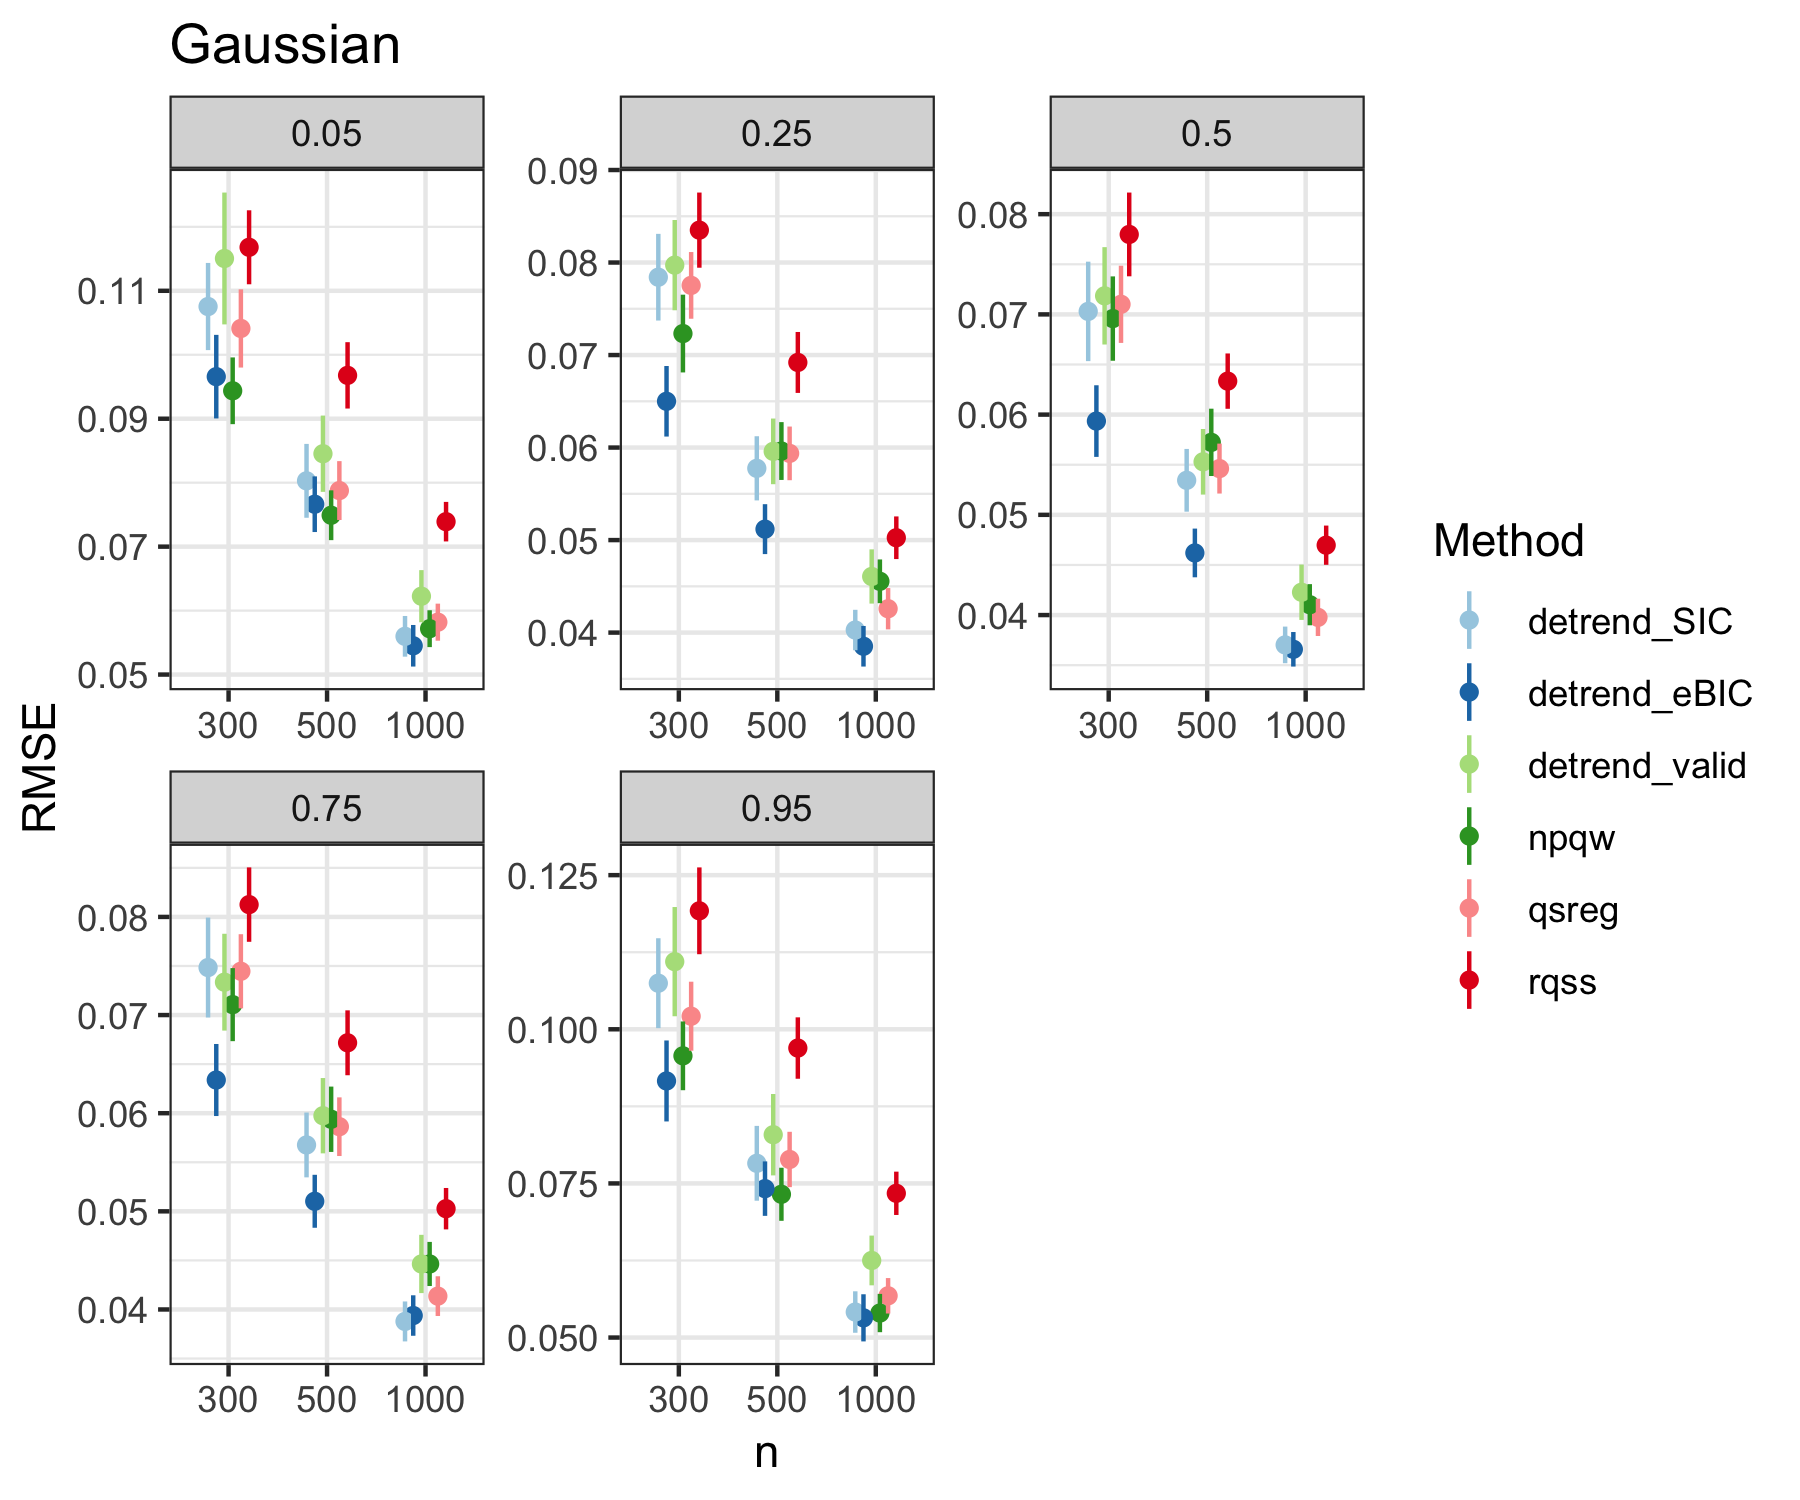
\includegraphics[width=\linewidth]{Figures/gaus_mse.png}	
		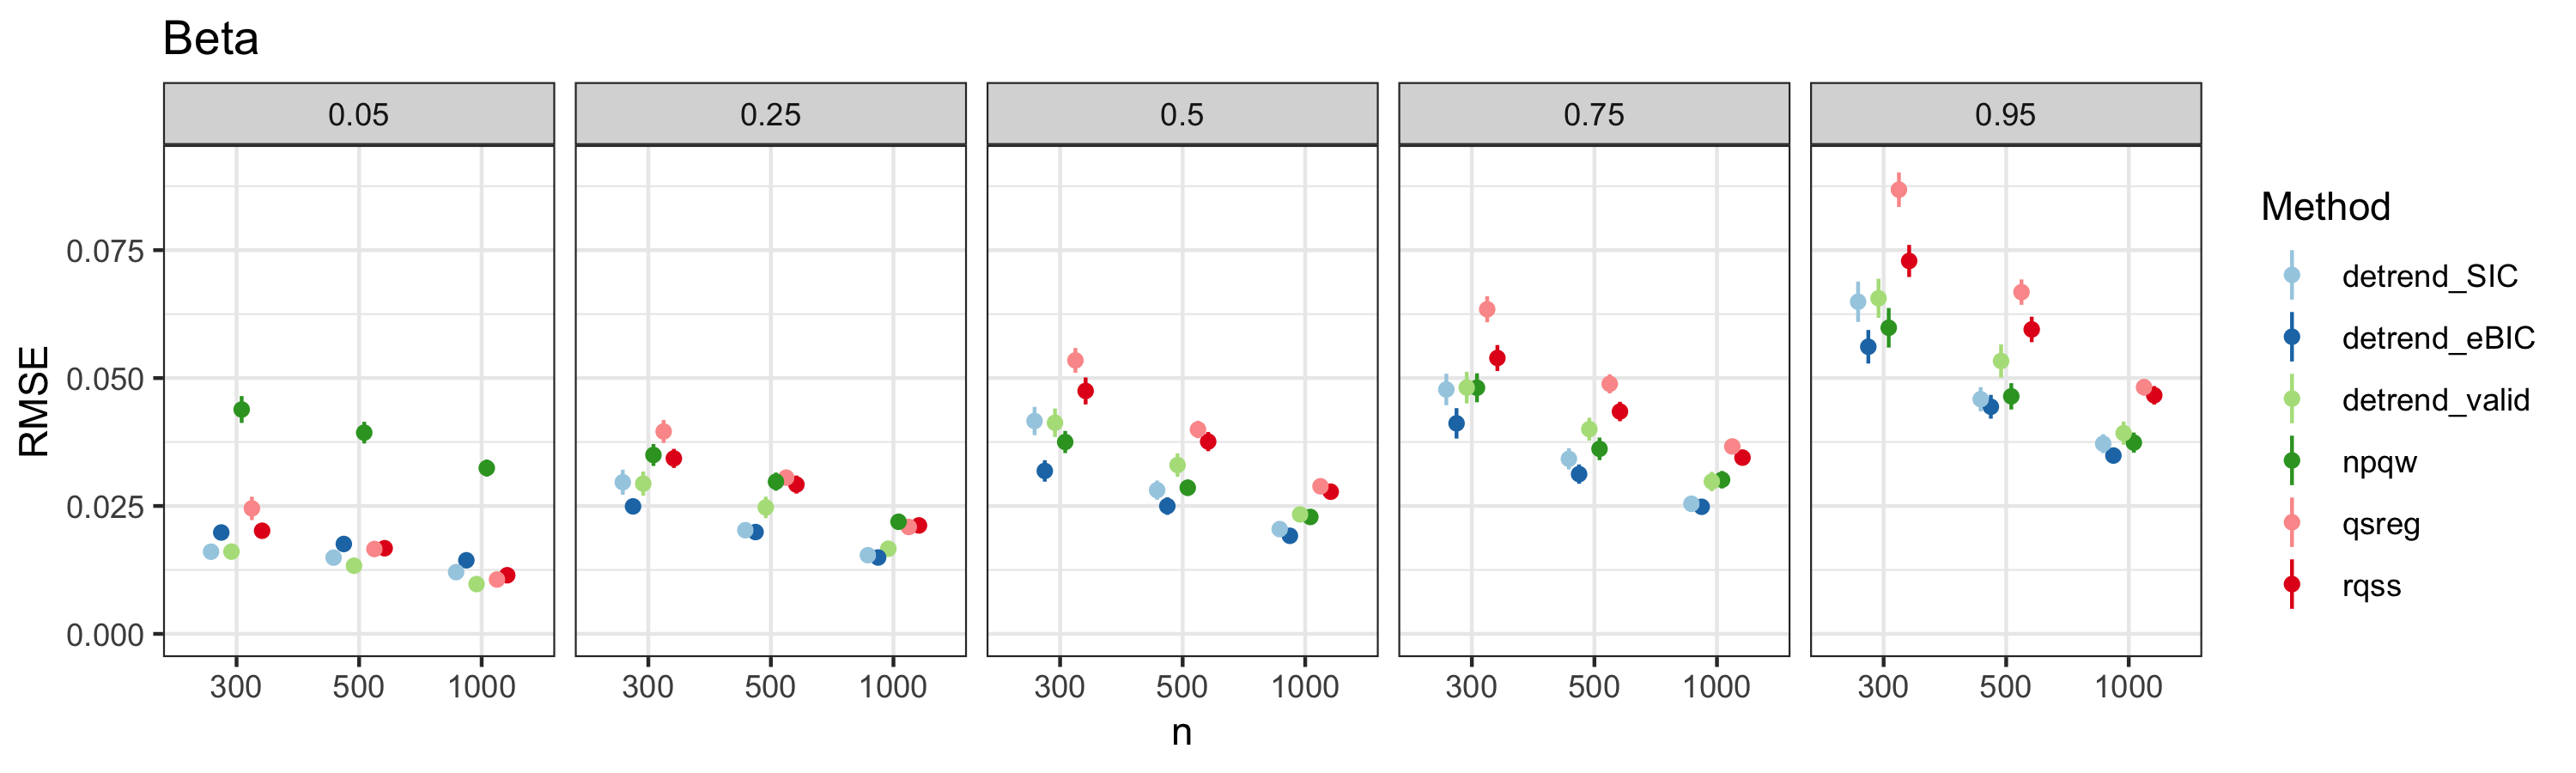
\includegraphics[width=\linewidth]{Figures/shapebeta_mse.png}
		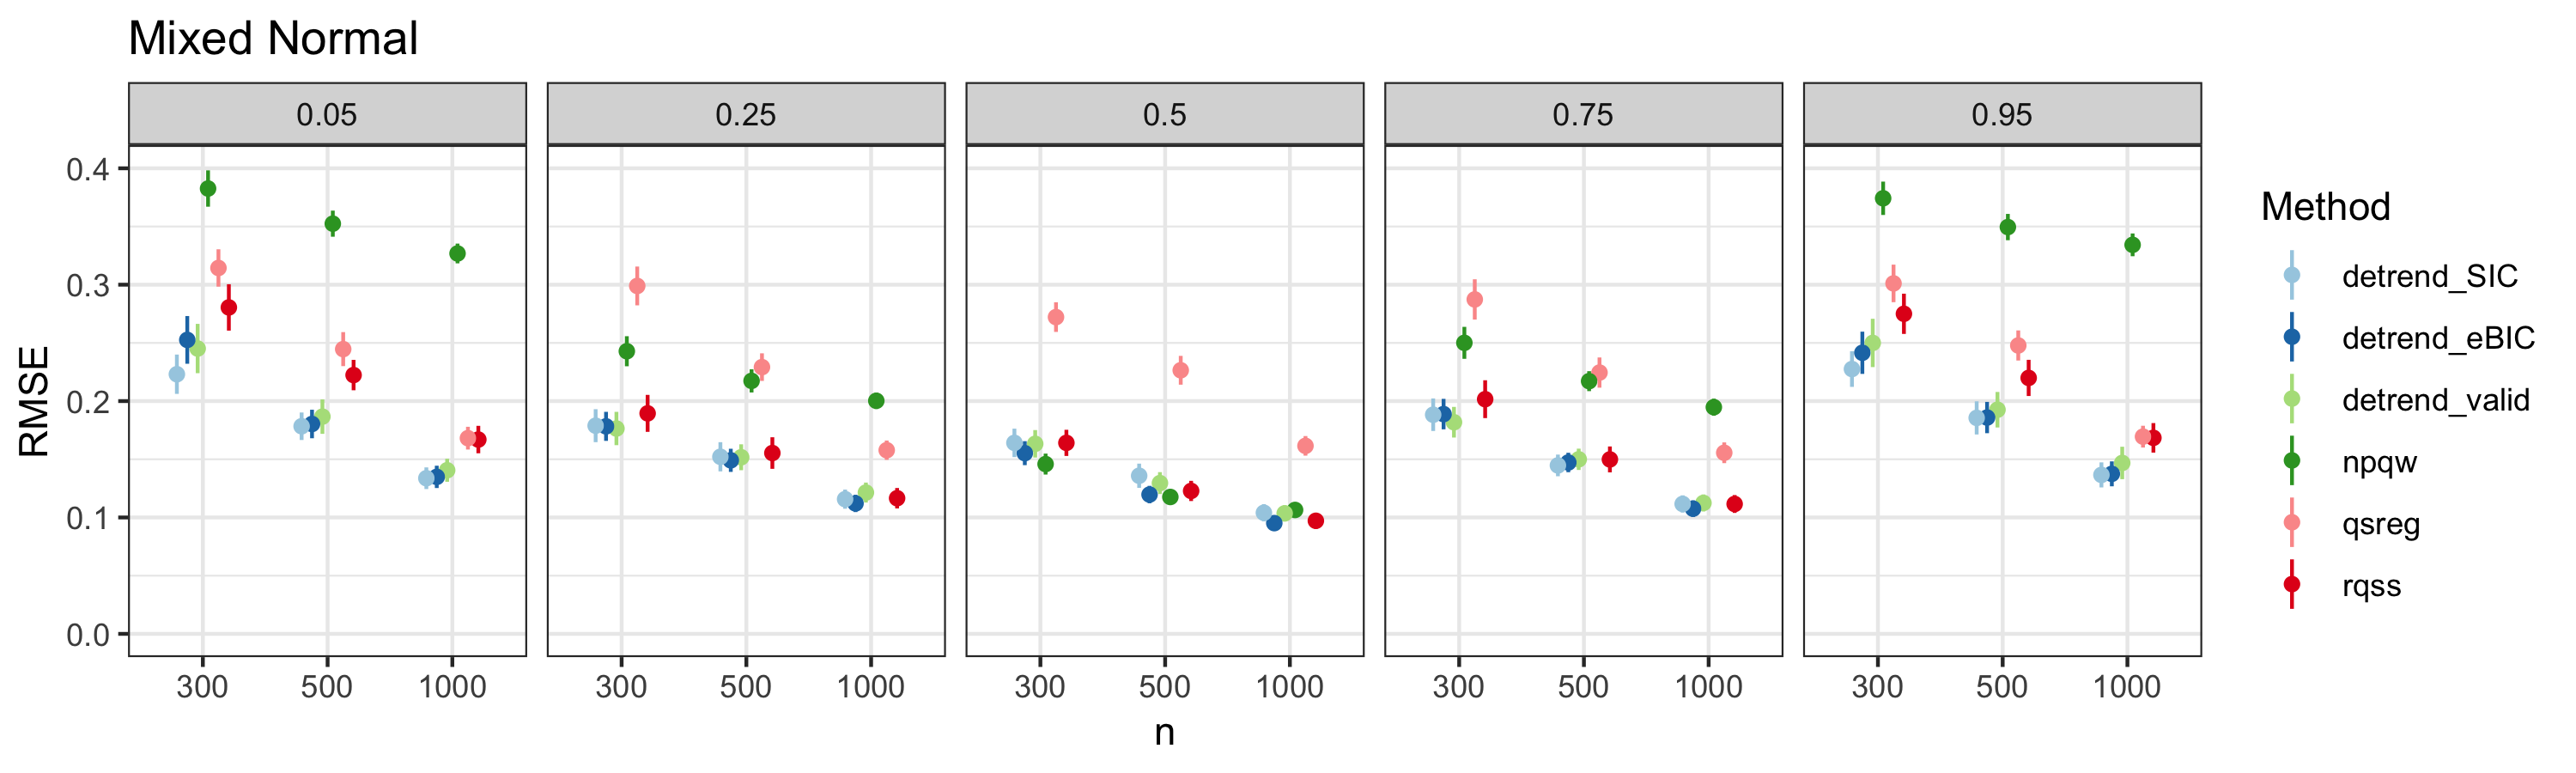
\includegraphics[width=\linewidth]{Figures/mixednorm_mse.png}
	\end{figure}
	In all of the designs the proposed detrend methods are either better than or comparable to existing methods. The npqw method performs particularly poorly in the mixed normal design, due to the fact that it assumes the data comes from a scale-location model which is violated in this case. 
	
	\subsection{Peak Detection}
	We use another simulation design based on the applied problem we aim to solve. We assume that the measured data can be represented by 
	\begin{equation}
	Y(t) = s(t) + b(t) + \epsilon(t)
	\end{equation} 
	where $s(t)$ is the true signal at time $t$, $b(t)$ is the drift component that varies smoothly over time and $\epsilon(t) \sim N(0, \sigma^2)$ is an error component. We assume $t$ is a uniformly spaced sequence of time points between 0 and 1. We generate $b(t)$ using a cubic natural spline basis function with degrees of freedom sampled from $n/50$ to $n/25$ with equal probability, and coefficients drawn from an exponential distribution with rate 1. The true signal function is assumed to be zero with Gaussian peaks. The number of peaks is sampled from $n/100$ to $n/50$ with equal probability with centers uniformly distributed between 0.1 and 0.9 and bandwidths uniformly distributed between $1/n$ and $5/n$ and areas uniformly distributed between 0 and $20/n$. One hundred datasets were generated for $n=\{300, 500, 1000, 5000\}$. We compare the methods ability to estimate the true quantiles of $b(t) + \epsilon$  for $\tau \in \{0.01, 0.05, 0.1\}$ and calculate the root mean squared error (RMSE). 
	
	\begin{figure}[h]
		\caption{Example of simulated peaks, baseline, and observed measurements.}
		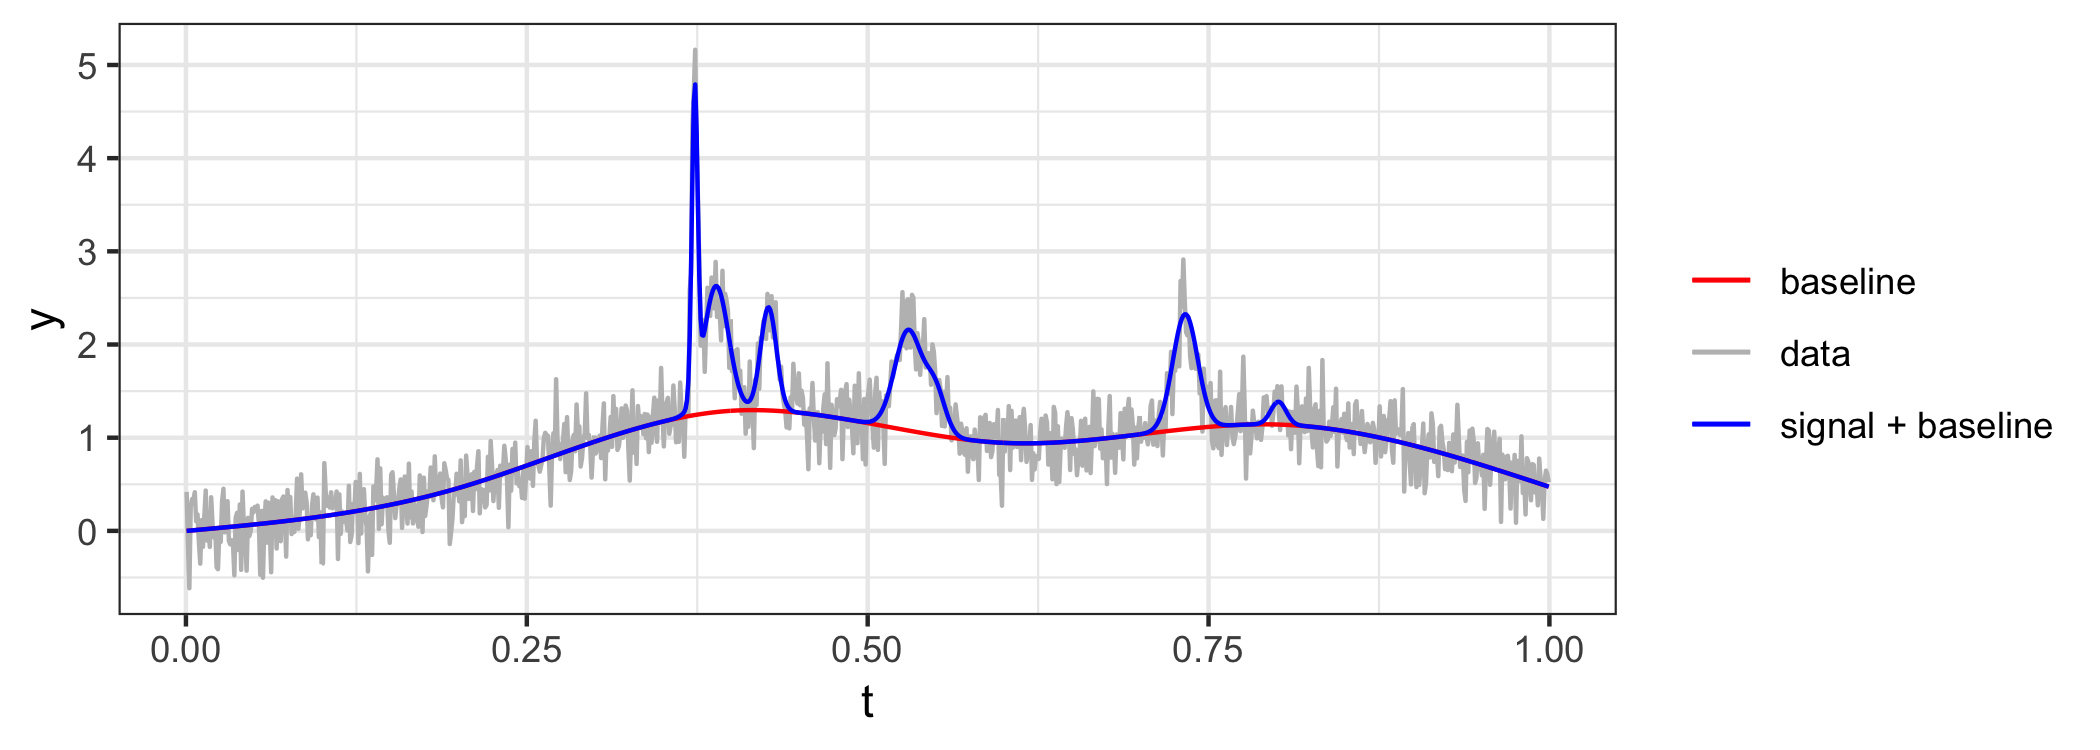
\includegraphics[width = \linewidth]{Figures/ex_peaks.png}
	\end{figure}

	In addition to the RMSE we also calculated the signal miss-classification rate. We first classified the ``true" peaks function into signal or not based on a threshold of 0.1. We then classified the detrended data using three different thresholds and calculated the fraction miss-classified. An illustration of the observations classified as signal after detrending compared to the ``true signal" is shown in Fig. 9. 
	
	
	Our detrend\_BIC method performs the best overall in terms of both RMSE and miss-classification rate. The lowest miss-classification rates were obtained using the detrend\_eBIC method and a threshold of 1 for all data sizes. While qsreg was competitive with our method in some cases, both the RMSE and miss-classification rate increased substantially with the size of the dataset. 
	
	\begin{figure}[h!]
		\caption{Example signal classification using threshold. Red indicates true signal $>0.1$, blue indicates classified as signal after baseline removal using eBIC detrendr and a threshold of 1.}
		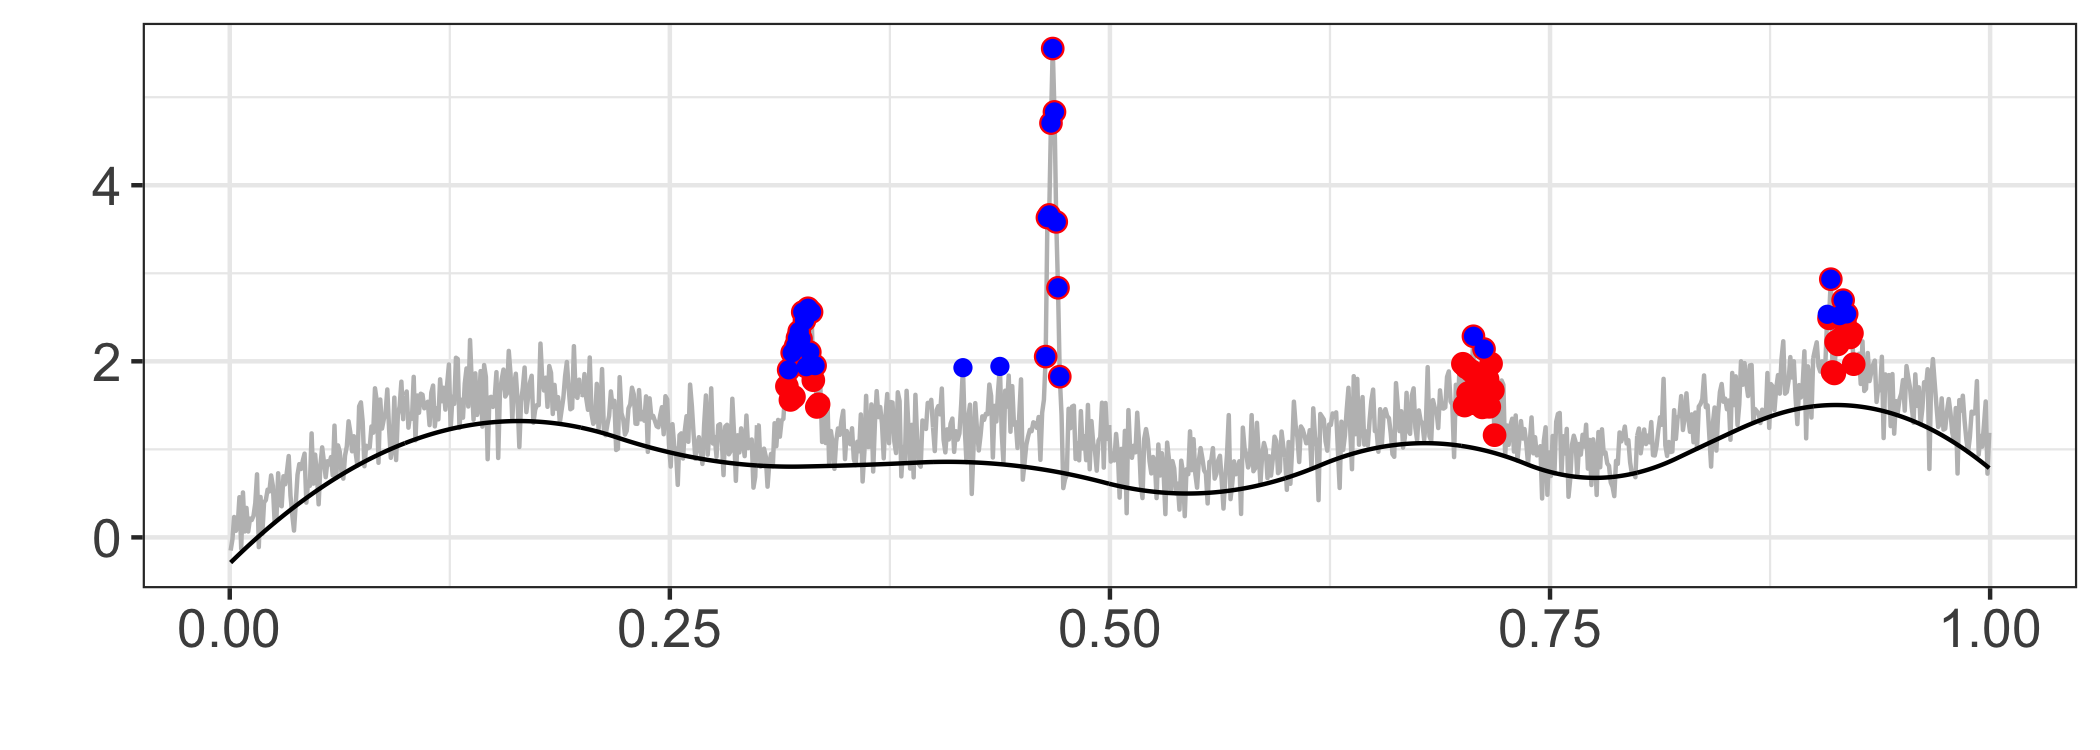
\includegraphics[width = \linewidth]{Figures/peaks_eg_class.png}
	\end{figure}
	

	\begin{figure}[h!]
		\caption{Class averaged accuracy by threshold, data size, and method (1 is best 0.5 is worst).}
		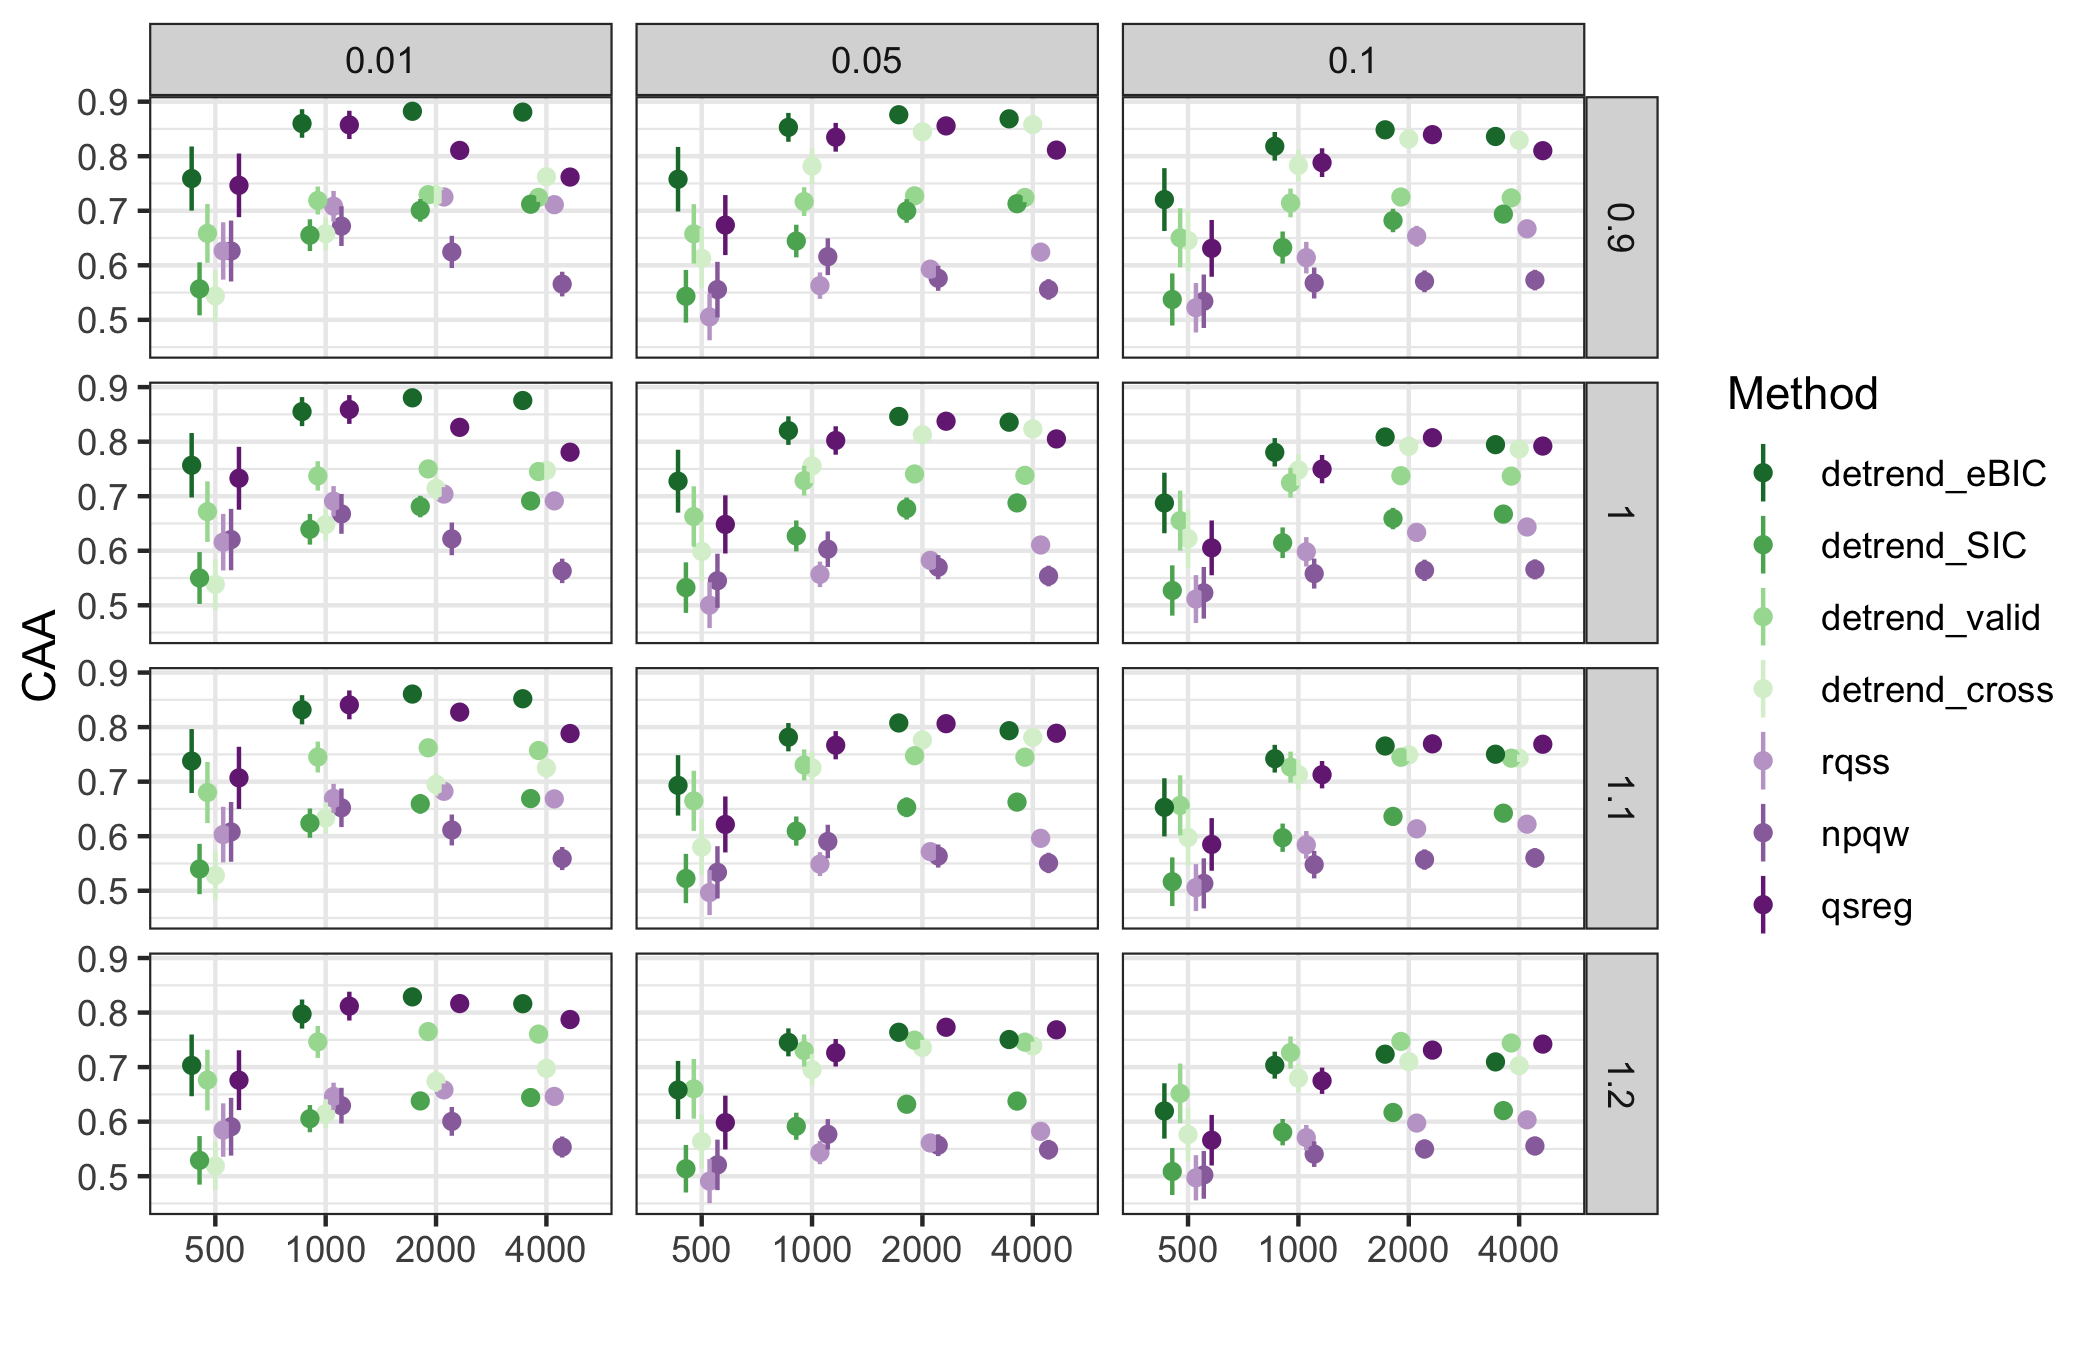
\includegraphics[width = \linewidth]{Figures/peaks_CAA.png}
	\end{figure}


	\FloatBarrier
	
	\section{Application}
	
	
	Our windowed detrend method was used to removed the baseline drift from low cost air quality sensors so that the signal could be categorized using a simple threshold. The measurements were first standardized to have mean zero and variance 1. Three quantile levels for estimating the baseline trend were compared. The total dataset consisted of 52,322 observations per node. 
	The signal thresholds were set using the first 15,000 observations where it was known no signal was present. The thresholds were set as 3 times the standard deviation plus the mean of observations in this time period. The total number of seconds of signal for each node as well as the number of seconds where multiple nodes both reported signal is shown in Table 1. Table 2 shows the fraction of observations with different signal classifications by node combination. 
	
	\begin{figure}
		\caption{Low cost sensor data before drift removal (top), after drift removal using windowed detrend with eBIC (middle), 
			and zoomed in on signal area (bottom). Horizontal lines represent signal thresholds.}
		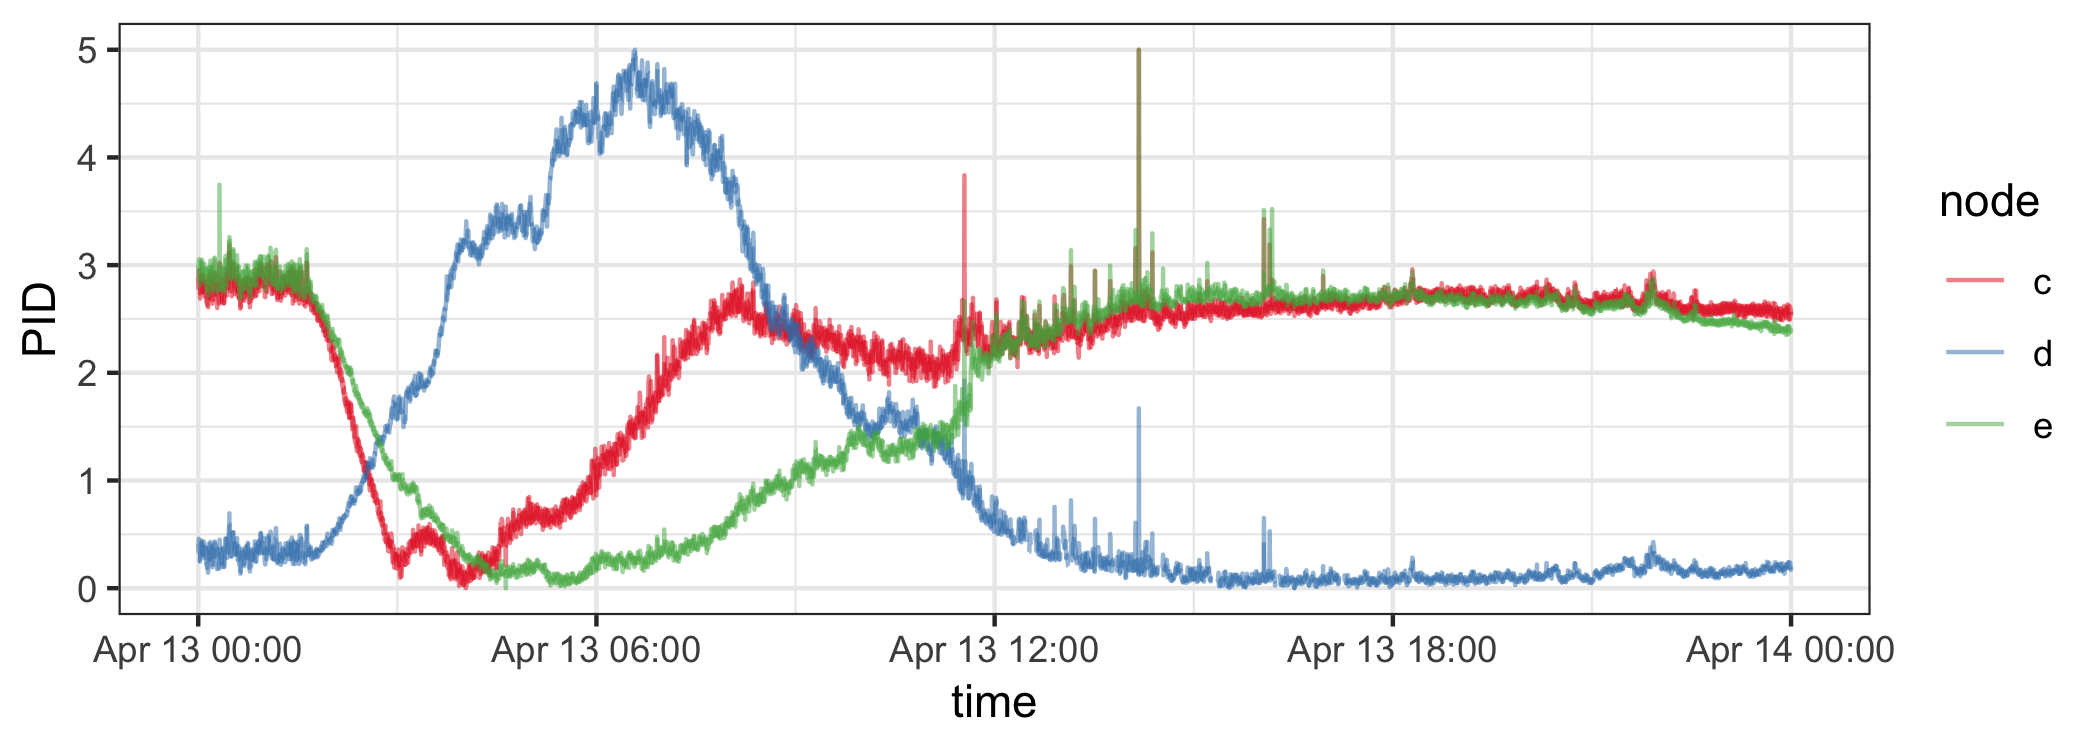
\includegraphics[width = \linewidth]{Figures/uncorrected_data.png}
		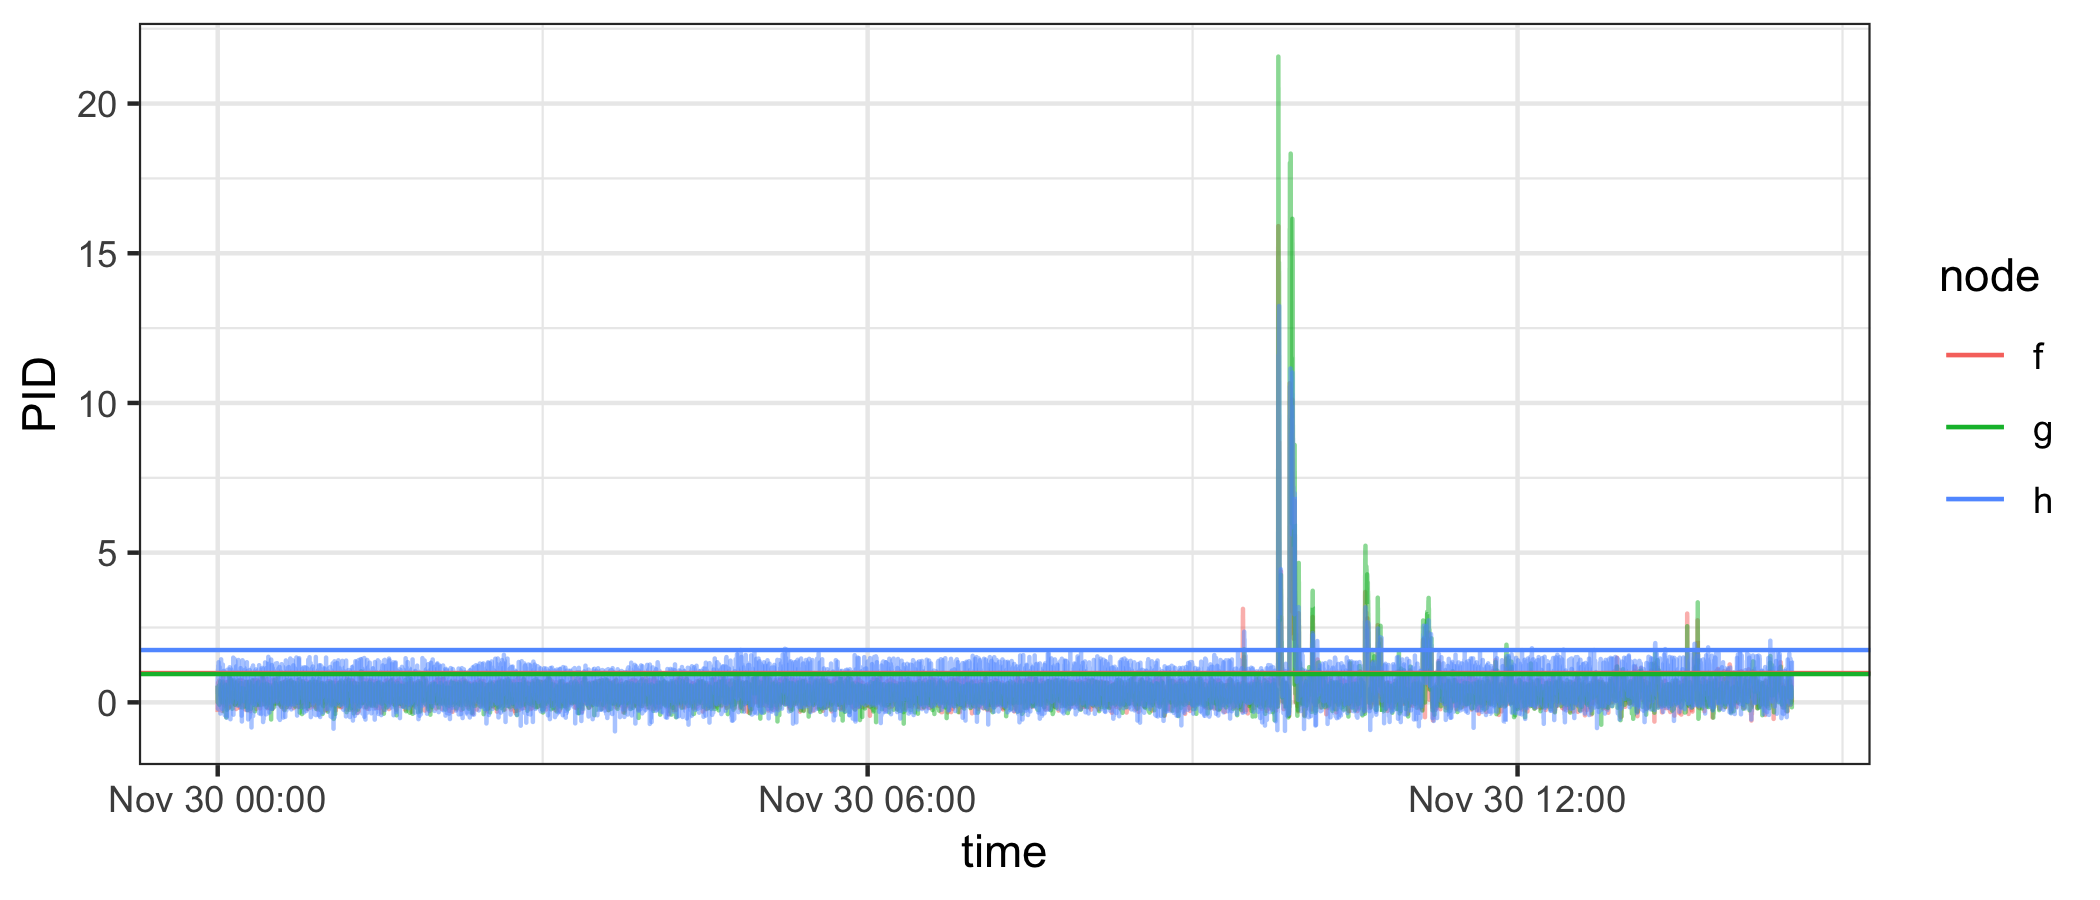
\includegraphics[width = \linewidth]{Figures/corrected_data.png}
		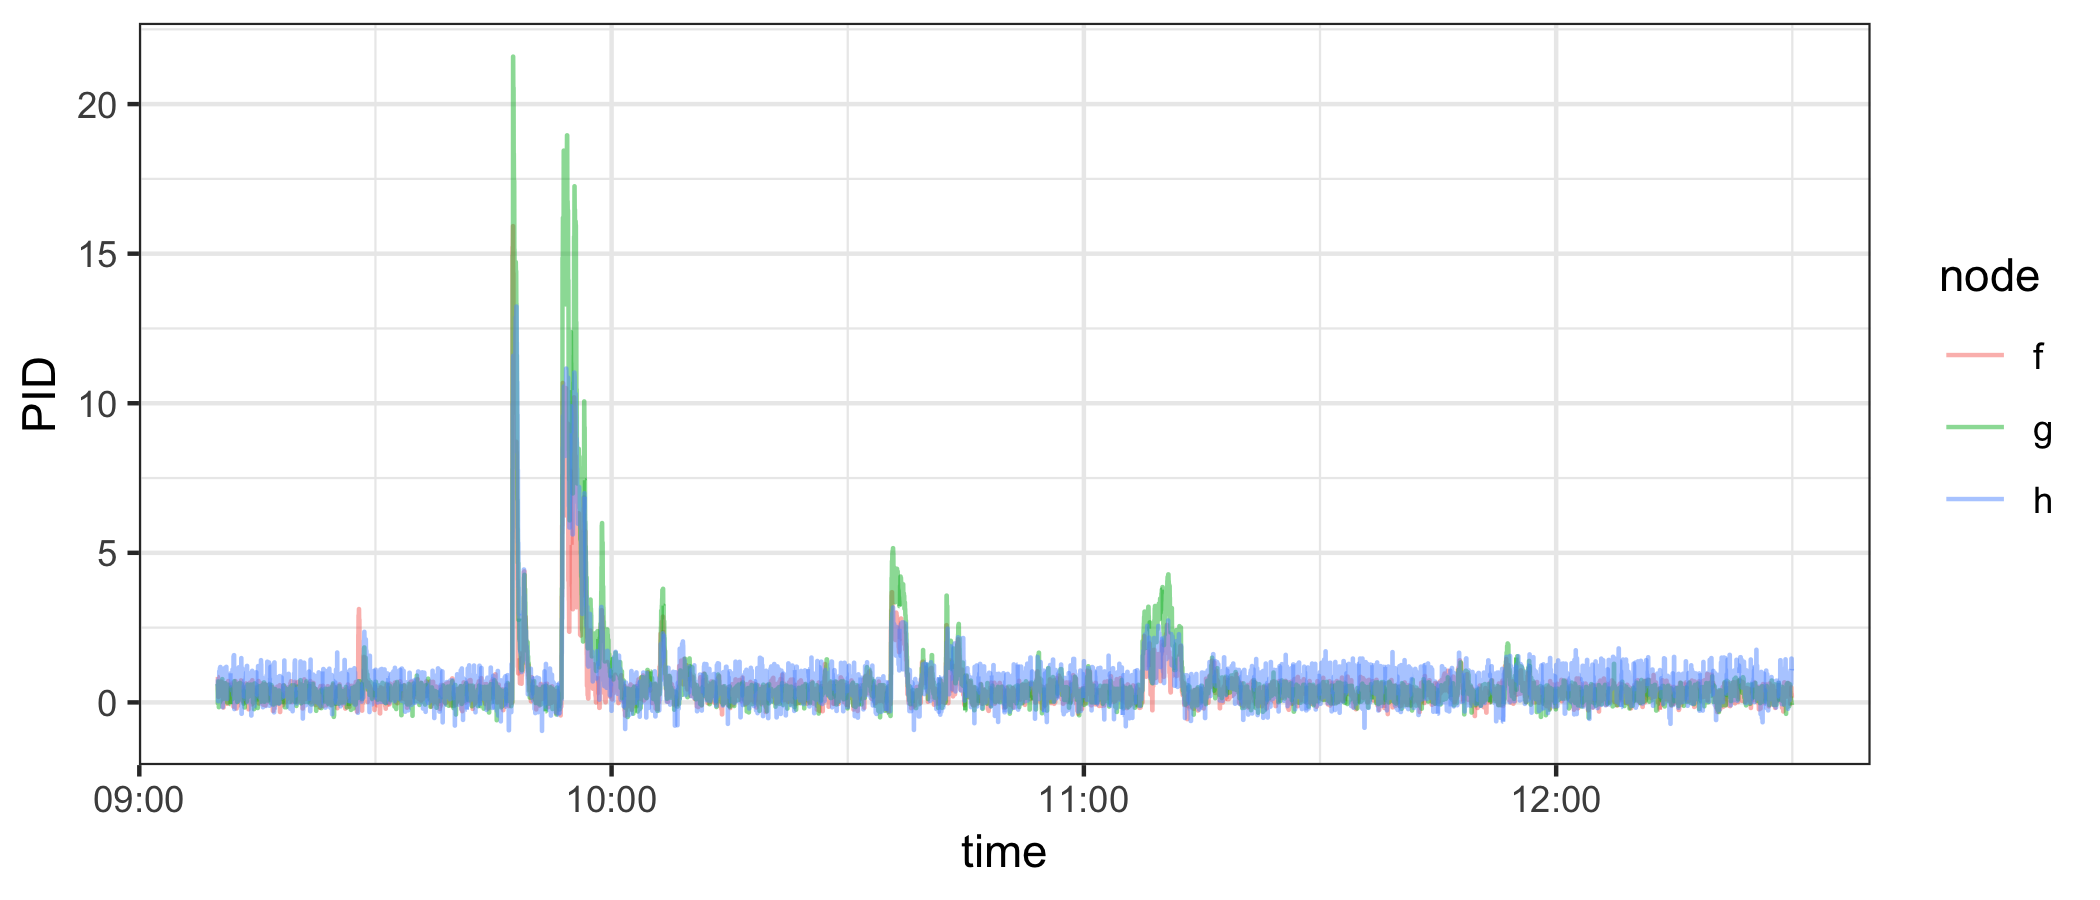
\includegraphics[width = \linewidth]{Figures/corrected_zoom_data.png}
	\end{figure}

	%latex.default(conf_out, file = "../Manuscript/complete_confusion.tex",     rowlabel = "", rowname = c("f = 0", "f = 1"), cgroup = c("h = 0",         "h = 1"), colheads = rep(c("g = 0", "g = 1"), 2), n.cgroup = c(2,         2), caption = "Confusion matrices for 3 SPod nodes after baseline removal.")%
\begin{table}[!tbp]
\caption{Confusion matrices for 3 SPod nodes after baseline removal.\label{conf}} 
\begin{center}
\begin{tabular}{lrrcrr}
\hline\hline
\multicolumn{1}{l}{\bfseries }&\multicolumn{2}{c}{\bfseries h = 0}&\multicolumn{1}{c}{\bfseries }&\multicolumn{2}{c}{\bfseries h = 1}\tabularnewline
\cline{2-3} \cline{5-6}
\multicolumn{1}{l}{}&\multicolumn{1}{c}{g = 0}&\multicolumn{1}{c}{g = 1}&\multicolumn{1}{c}{}&\multicolumn{1}{c}{g = 0}&\multicolumn{1}{c}{g = 1}\tabularnewline
\hline
f = 0&$51123$&$386$&&$ 3$&$ 29$\tabularnewline
f = 1&$  108$&$318$&&$16$&$337$\tabularnewline
\hline
\end{tabular}\end{center}
\end{table}
	
	
	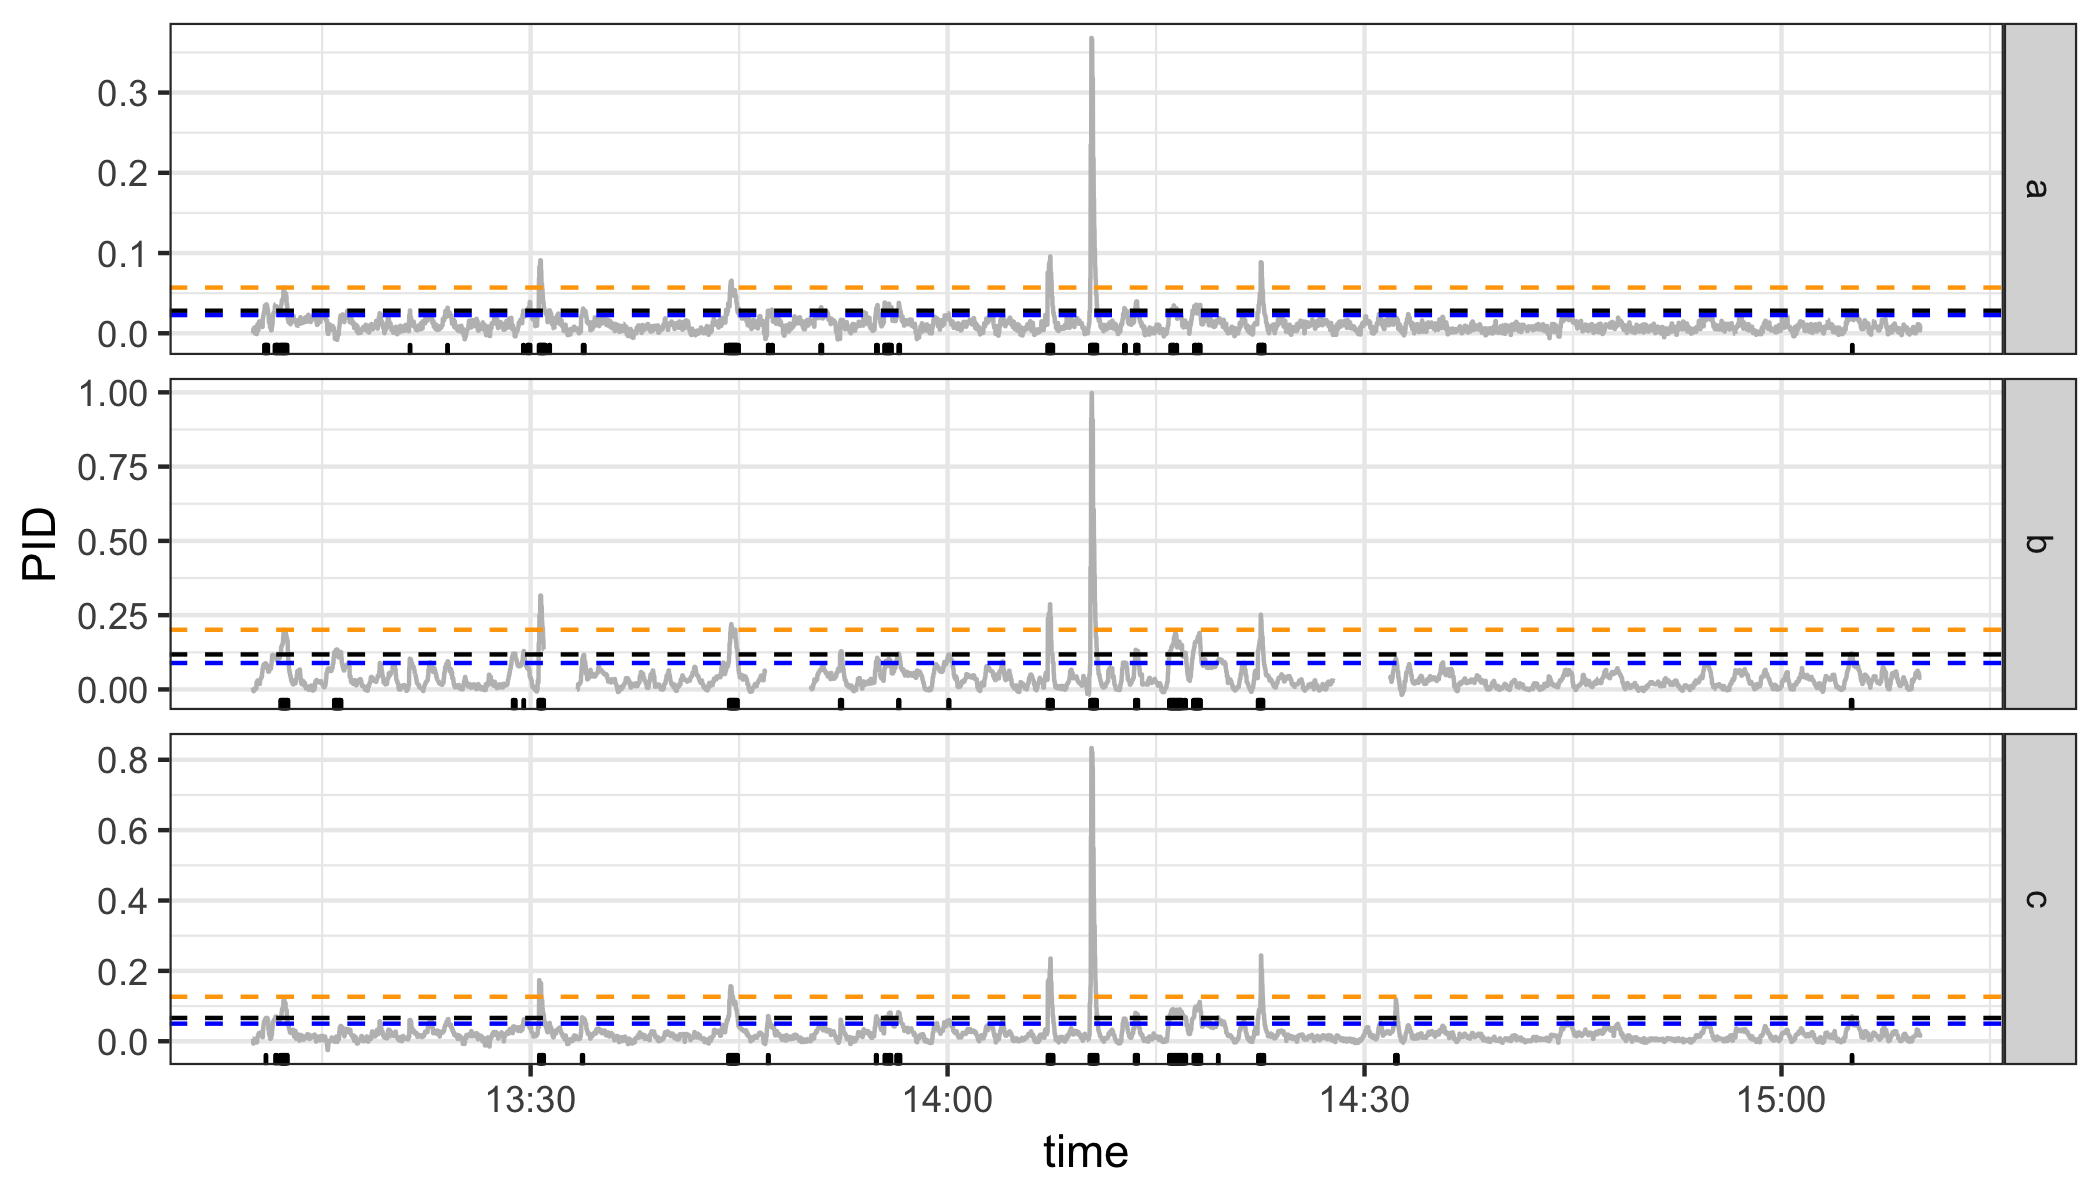
\includegraphics[width = \linewidth]{Figures/corrected_rugplot.png}

	\section{Conclusion}
	\label{sec:conc}
	
	
	\bigskip
	\begin{center}
		{\large\bf SUPPLEMENTARY MATERIAL}
	\end{center}
	
	\begin{description}
		
		\item[R-package for detrend routine:] R-package detrendr containing code to perform the diagnostic methods described in the article. The package also contains all datasets used as examples in the article. (GNU zipped tar file)
				
	\end{description}
	
	\section{References}

	
	\bibliographystyle{asa}
	\bibliography{detrendify}
	
\end{document}

